\documentclass[12pt,a4paper]{article}

\usepackage[utf8]{inputenc}
\usepackage[brazilian]{babel}
\usepackage{amsmath}
\usepackage{graphicx}
\usepackage{longtable}
\usepackage{siunitx}
\usepackage{booktabs}
\usepackage{geometry}
\usepackage{float}
\usepackage{indentfirst}
\usepackage{newtxtext}
\usepackage{newtxmath}

\usepackage[authoryear]{natbib}

\geometry{margin=2.5cm}

\title{Determinação do momento de Inércia de um corpo rígido.}
\author{Enzo Rocha Leite Diniz Ribas \\ Centro Federal de Educação Tecnológica de Minas Gerais}
\date{\today}

\begin{document}
\begin{titlepage}

\begin{center}


\includegraphics[width=4cm]{media/Logo_CEFET-MG.png}

\Large
Centro Federal de Educação Tecnológica de Minas Gerais

\vspace{1cm}

\Large
Curso de Engenharia Mecânica

\vspace{2cm}

\Huge
Determinação do momento de Inércia de um corpo rígido.

\vspace{3cm}

\begin{flushright}
\Large
Mecânica, Oscilações, Fluidos e Termodinâmica, Turma T03 \\
Prof. Dr. Mauro Lucio Lobão Iannini
\end{flushright}

\vspace{3cm}

\large
Enzo Rocha Leite Diniz Ribas (Eng. Mecânica - 20253002819)\\
Gabriel Resende Amorim Oliveira (Eng. Elétrica - 20233014438)\\
Leandro Césari e Silva Barros (Eng. Mecânica - 20253005104)\\

\vfill

\Large
Belo Horizonte

\Large
\the\year/{1}

\end{center}

\end{titlepage}

\section{Introdução}

O roteiro do experimento \citep{Roteiro_Experimento_04} propõe a determinação do momento de inércia de um corpo rígido acoplado a uma polia, por meio da análise do movimento causado pela descida de uma massa pendente.

\section{Fundamentação Teórica}
O momento de inércia de um corpo rígido em relação a um eixo de rotação, tem um papel análogo ao da massa no movimento de translação, isto é, representa a \textit{inércia de rotação} \citep{moyses2013}. Para corpos de densidade de massa constante, o momento de inércia é dado por
\begin{equation}
    I = \int_{\mathcal{Q}} r^2 \, dm,
    \label{eq:moment_inertia}
\end{equation}
em que \textit{r} é a distância do elemento de massa $dm$ ao eixo de rotação e $\mathcal{Q}$ é região ocupada pelo corpo no espaço. No caso de um sólido tridimensional, seu momento de inércia é dado por
\begin{equation}
    I = \iiint_{V} r^2 \, \rho(r) dV,
    \label{eq:moment_inertia}
\end{equation} 
em que \textit{V} é a região do volume do corpo, e $\rho$ é a sua densidade de massa em função da posição.

O disco utilizado no experimento é um corpo rígido de densidade de massa constante, e seu momento de inércia em relação ao eixo de rotação é dado por
\begin{equation}
    I_{disco} = \frac{1}{2} m_{disco} \times r_{disco}^2,
    \label{eq:moment_inertia_disk}
\end{equation}~\cite{moyses2013}.

Com base no diagrama de corpo livre do sistema (Figura~\ref{fig:free_body_diagram}), é possível encontrar uma expressão que relacione o momento de inércia do sistema com a aceleração angular $\alpha$ do disco, a massa pendente $m$, a aceleração da gravidade $g$ e o raio da polia $r_p$.

\begin{figure}[H]
\centering
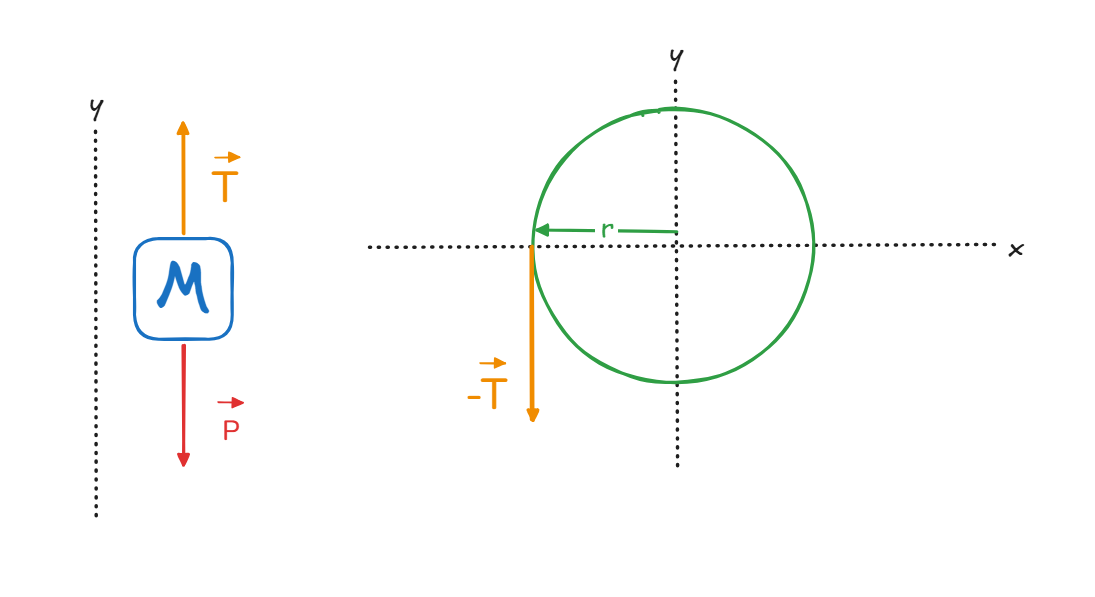
\includegraphics[width=0.8\textwidth]{media/photos/sistema/freebody_diagram}
\caption{Sistema de queda utilizado para a determinação do momento de inércia. Fonte: Autor}
\label{fig:free_body_diagram}
\end{figure}

Assumindo para cima como a direção positiva, e o sentido antihorário como o sentido positivo de rotação, além disso considerando que o fio não escorrega na polia, pela segunda lei de Newton temos:

\begin{align}
    \vec{F_{net}} &= m \vec{a} \nonumber \\
    \implies  \vec{T} + \vec{P} &= m\vec{a} \nonumber \\
    \vec{T} - mg\hat{\jmath} &= m\vec{a} \nonumber \\
    T - mg &= ma_y \label{eq:net_force}
\end{align}

O torque $\vec{\uptau_T}$ causado pela força de tensão $\vec{T}$ na polia é dado por
\begin{align}
    \vec{\uptau_T} &= \vec{r_p} \times \vec{T} \nonumber \\
    &= r_p T \hat{k}, \label{eq:torque}
\end{align}

Pela segunda lei de Newton para rotação, temos
\begin{align}
    \vec{\uptau_{net}} &= I \vec{\alpha} \nonumber \\
\end{align}

Substituindo a expressão do torque $\vec{\uptau_T}$ da equação \eqref{eq:torque} na equação da segunda lei de Newton para rotação, temos

\begin{align}
    \vec{\uptau_T} &= I \vec{\alpha} \nonumber \\
    r_p T \hat{k} &= I \alpha \hat{k} \nonumber \\
    r_p T &= I \alpha. \label{eq:net_torque}
\end{align}

A aceleração tangecial do disco é dada por
\begin{align}
    \vec{a_t} &= \vec{\alpha} \times \vec{r_p} \nonumber \\
    &= \alpha \hat{k} \times -r_p \hat{\imath} \nonumber \\
    &= -\alpha r_p \hat{\jmath}. \label{eq:tangential_acceleration}
\end{align}

Isolando a tração $T$ da equação \eqref{eq:net_torque} e substituindo $T$ e $a_y$ na equação \eqref{eq:net_force}, temos

\begin{align}
    T &= \frac{I \alpha}{r_p} \nonumber \\
    \implies \frac{I \alpha}{r_p} - mg &= m (-\alpha r_p) \nonumber \\
    - mg &= m (-\alpha r_p) - \frac{I \alpha}{r_p}  \nonumber \\
    mg &= m (\alpha r_p) + \frac{I \alpha}{r_p}  \nonumber \\
    mg &= \alpha r_p \left(m + \frac{I}{r_p^2}\right) \nonumber \\
    \frac{1}{r_p}\frac{mg}{\left(m + \frac{I}{r_p^2}\right)} &= \alpha \nonumber \\
    \implies \alpha &= \frac{1}{r_p}\frac{g}{\left(1 + \frac{I}{mr_p^2}\right)} \label{eq:angular_acceleration}
\end{align}

Sabemos que a aceleração angular $\alpha$ é a derivada de segunda ordem da posição angular $\theta$ do disco em função do tempo, ou seja, $\alpha = \frac{d^2\theta}{dt^2}$.

\begin{align}
    \alpha = \frac{d^2\theta}{dt^2} = \frac{d}{dt}\frac{d\theta}{dt} &= \frac{d\omega}{dt} \nonumber \\
    \int_0^t \alpha \, dt &= \int_{\omega(0)}^{\omega(t)} d\omega \nonumber \\
    \alpha t &= \omega(t) - \omega(0) \nonumber \\ 
    \implies \omega(t) &= \omega(0) + \alpha t \nonumber \\
    \int_0^t \omega(t) \, dt &= \int_{\theta(0)}^{\theta(t)} d\theta \nonumber\\
    \int_0^t \left(\omega(0) + \alpha t\right) dt &= \theta(t) - \theta(0) \nonumber \\
    \implies \theta(t) &= \theta(0) + \omega(0)t + \frac{1}{2}\alpha t^2 \nonumber
\end{align}

Considerando as condições iniciais de $\theta(0) = 0$ e $\frac{d\theta}{dt}(0) = 0$, a posição angular do disco em função do tempo é dada por
\begin{equation}
    \theta(t) = \frac{1}{2}\alpha t^2.~\label{eq:posicao_angular}
\end{equation}
Substituindo a expressão para a aceleração angular da equação \eqref{eq:angular_acceleration} na equação \eqref{eq:posicao_angular} obtemos:

\begin{align}
    \theta(t) = \frac{1}{2} \left(\frac{1}{r_p}\frac{g}{\left(1 + \frac{I}{mr_p^2}\right)}\right) t^2 \nonumber \\
    \theta(t) = \frac{1}{2r_p} \left(\frac{g}{\left(1 + \frac{I}{mr_p^2}\right)}\right) t^2 ~\label{eq:posicao_angular_final} 
\end{align}

A equação \eqref{eq:posicao_angular_final} relaciona a posição angular do disco em função do tempo com o momento de inércia do sistema, a massa pendente, a aceleração da gravidade e o raio da polia. Assim, a partir dos dados experimentais de $\theta(t)$, é possível determinar o momento de inércia $I_{total}$ do sistema. Com o momento de inércia do sistema, é possível determinar o momento de inércia da polia $I_{polia}$ subtraindo o momento de inércia do disco $I_{disco}$ do momento de inércia total do sistema, ou seja, 

\begin{equation}
    I_{polia} = I_{total} - I_{disco}~\label{eq:moment_inertia_polia},
\end{equation}
\cite{Roteiro_Experimento_04}.

\section{Metodologia}

O sistema utilizado para a realização do experimento é composto por um disco acoplado a uma polia, com um fio enrolado em torno da polia, e uma massa pendente na extremidade do fio. O sistema é configurado de forma que a massa pendente possa descer livremente, causando a rotação do disco e da polia. 

\begin{figure}[H]
\centering
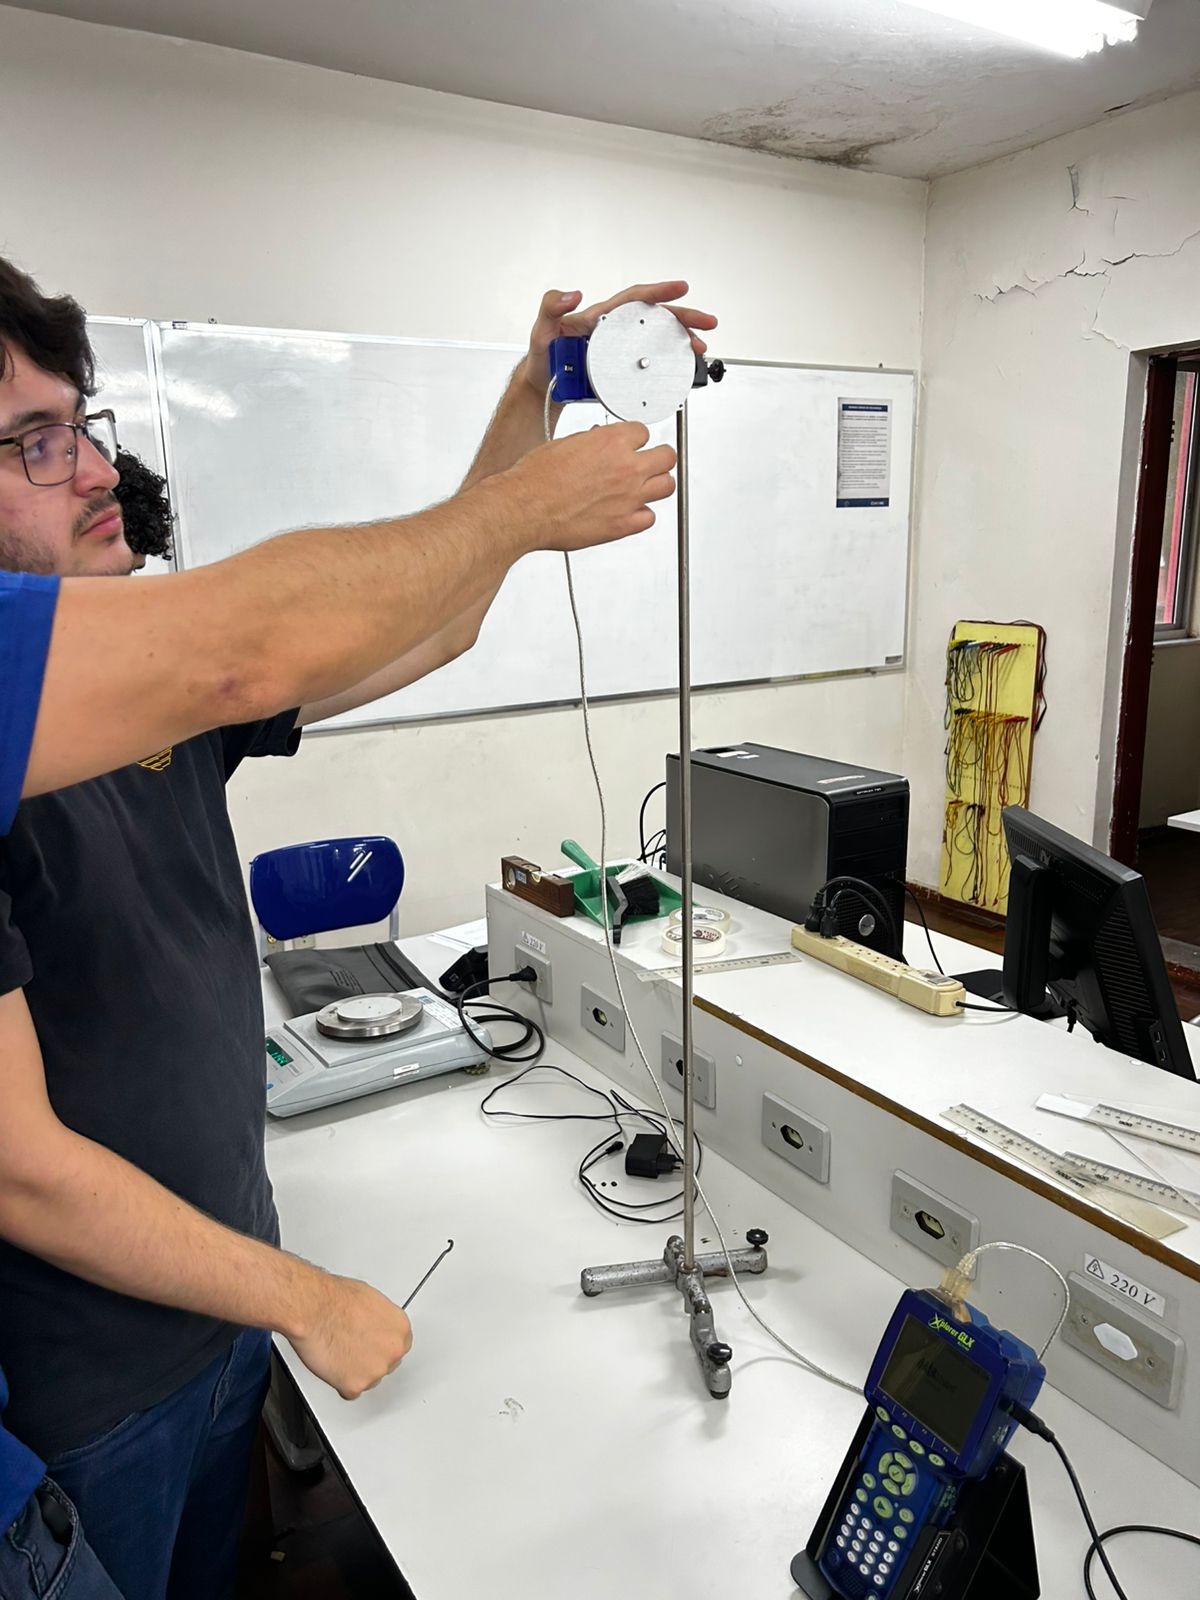
\includegraphics[width=0.4\textwidth]{media/photos/sistema_de_queda}
\caption{Sistema de queda utilizado para a determinação do momento de inércia. Fonte: Autor}
\label{fig:fall_setup}
\end{figure}

\begin{figure}[H]
\centering
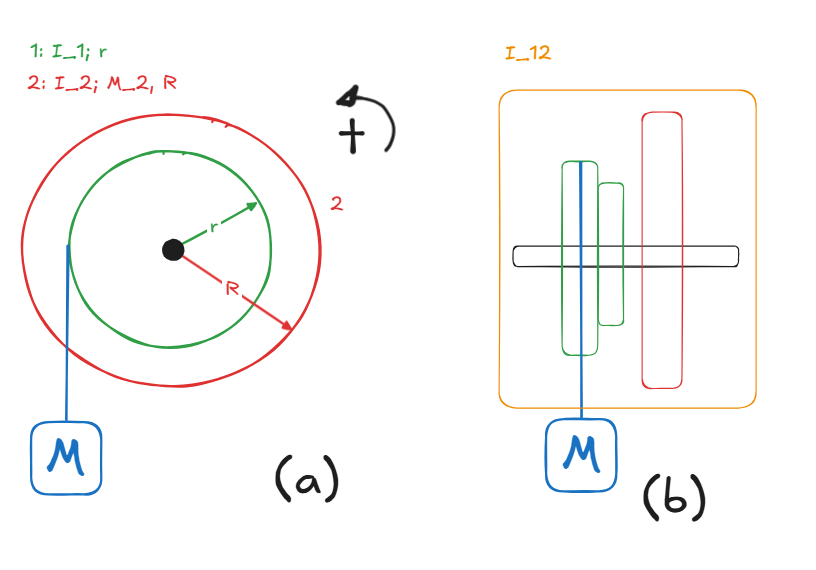
\includegraphics[width=0.8\textwidth]{media/photos/sistema/sistema_diagram}
\caption{Diagrama do sistema de queda utilizado para a determinação do momento de inércia. (a) Vista frontal do sistema, (b) Vista lateral do sistema. Fonte: Autor}
\label{fig:diagram_fall_setup}
\end{figure}

\begin{figure}[H]
\centering
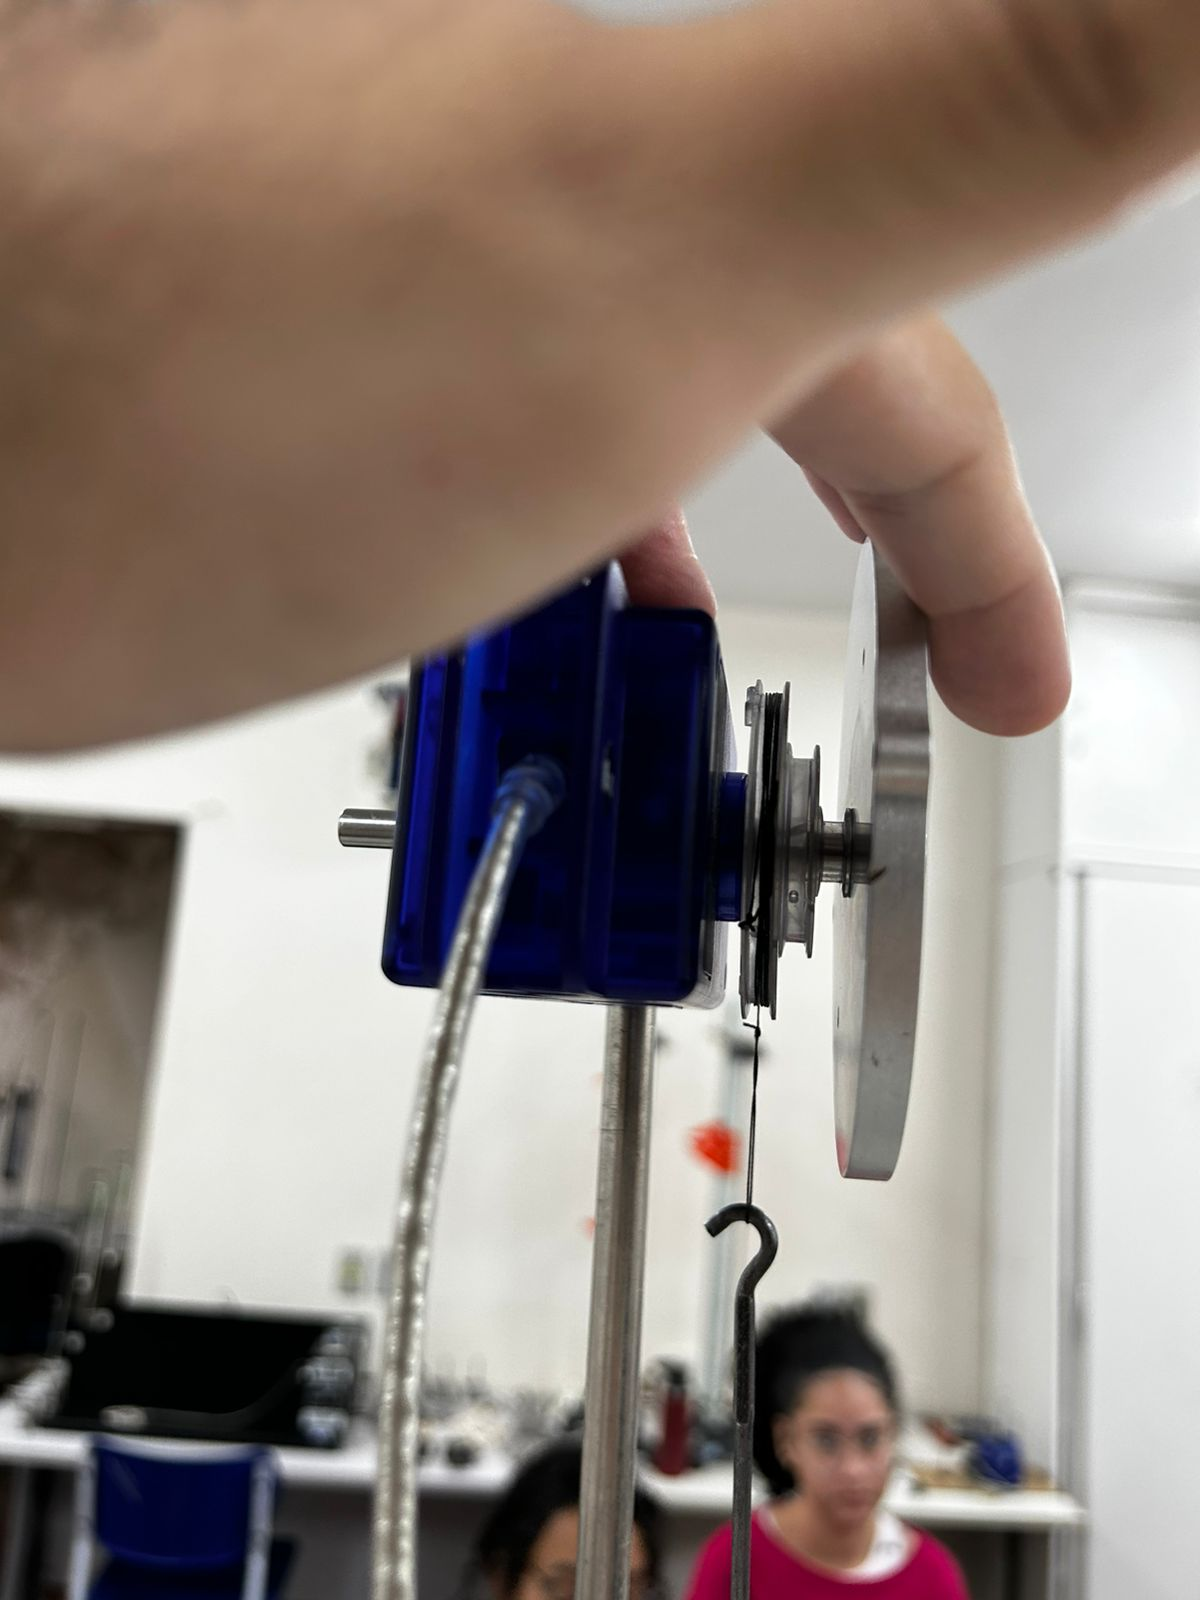
\includegraphics[width=0.4\textwidth]{media/photos/roldanas}
\caption{Conjunto de polias acopladas. A polia maior é utilizada para enrolar o fio. Fonte: Autor}
\label{fig:roldanas}
\end{figure}

Junto ao sistema, um coletor de dados (Figura~\ref{datalogger}) é utilizado para registrar a posição angular do disco em função do tempo, que será utilizada para a determinação do momento de inércia do sistema.

\begin{figure}[H]
\centering
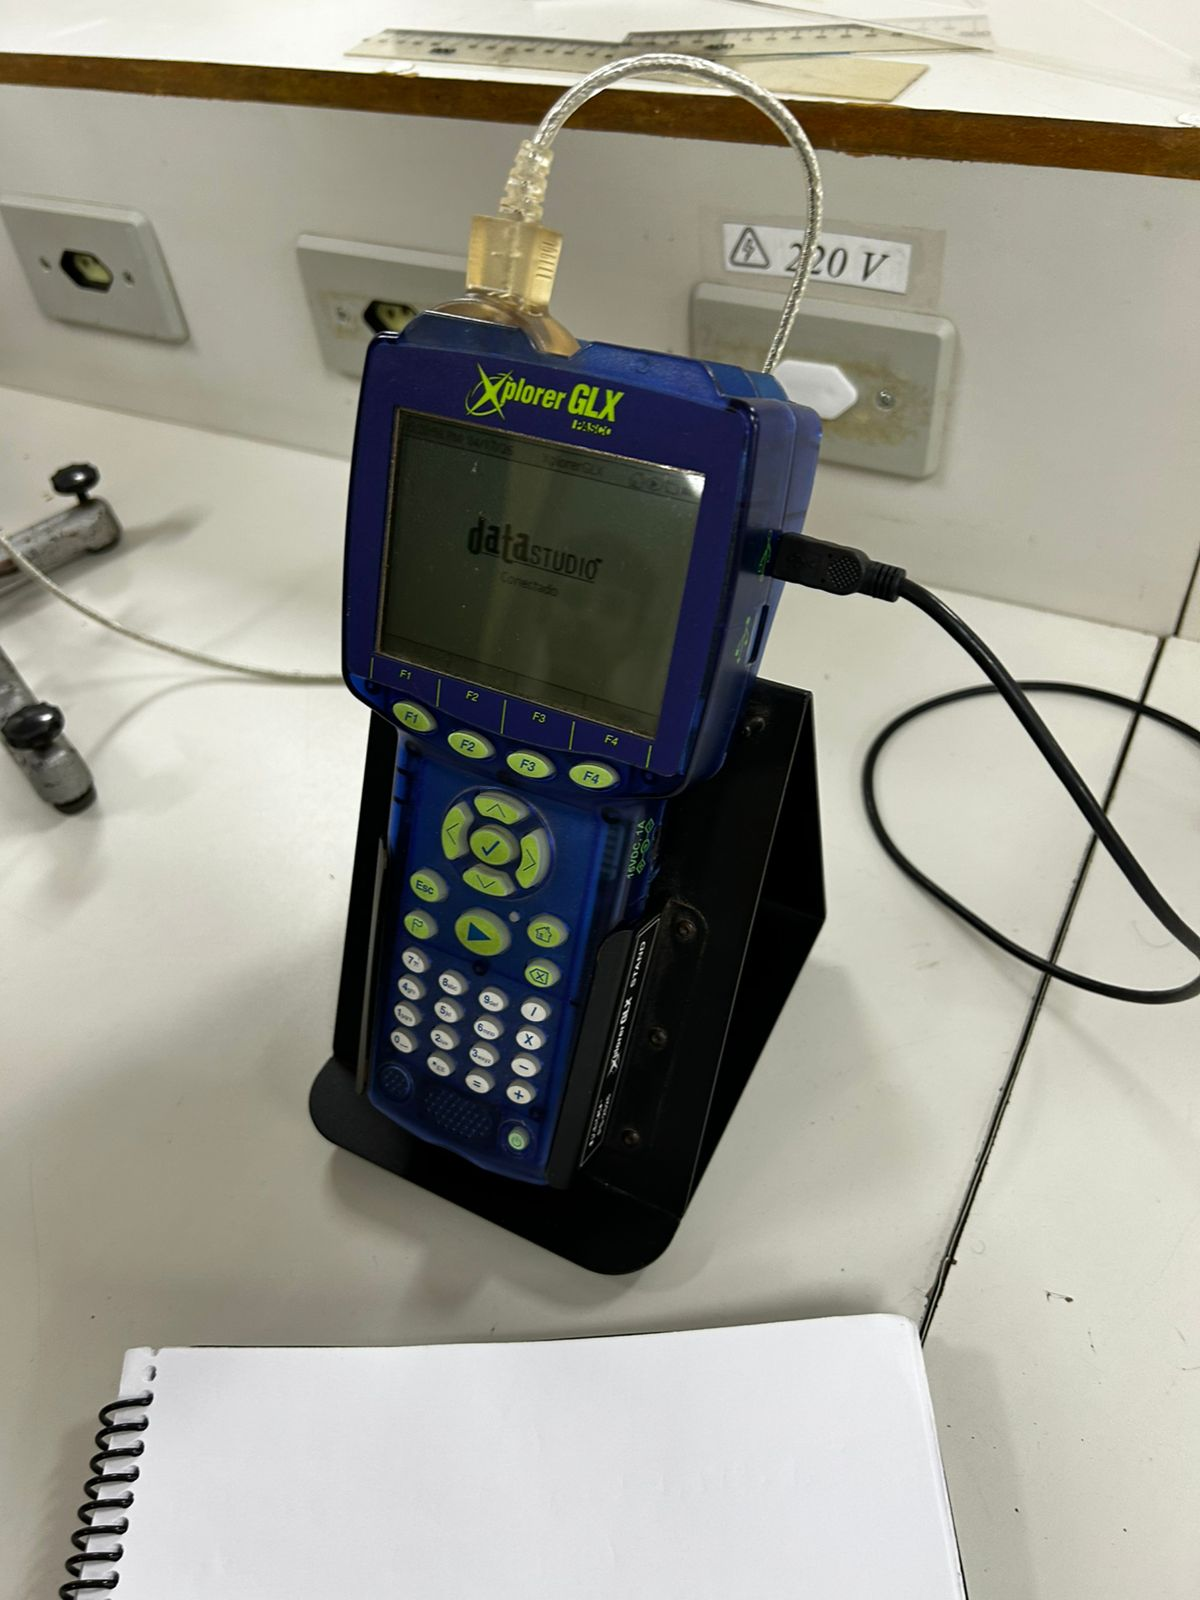
\includegraphics[width=0.7\textwidth]{media/photos/equipamentos/datalogger}
\caption{Coletor de dados utilizado para registrar a posição angular do disco em função do tempo. Fonte: Autor}~\label{datalogger}
\end{figure}

Através do ajuste da posição angular do disco em função do tempo feito no SciDAVis, utilizando a equação \eqref{eq:posicao_angular_final}, é possível determinar o momento de inércia do sistema, e consequentemente o momento de inércia da polia.

Considerando o caso geral, o ajuste linear da posição angular do disco em função do tempo é dado por
\begin{equation}
    \theta(t) = A t^2 + B t + C,~\label{eq:angular_position_geral}
\end{equation}

ou, no caso partindo do repouso,

\begin{equation}
    \theta(t) = A t^2,~\label{eq:angular_position_repouso}
\end{equation}

em que $A$, $B$ e $C$ são os coeficientes do ajuste. Comparando a equação do ajuste linear com a equação \eqref{eq:posicao_angular_final}, é possível perceber que o coeficiente $A$ do ajuste linear é dado por
\begin{align}
    A &= \frac{1}{2r_p} \left(\frac{g}{\left(1 + \frac{I}{mr_p^2}\right)}\right) \nonumber \\
    \implies I &= mr_p^2 \left(\frac{g}{2r_p A} - 1\right) \label{eq:moment_inertia_final}
\end{align}

\section{Procedimentos}

O procedimento experimental seguiu as seguintes etapas:

\subsubsection{Medida da Posição Angular em Função do Tempo}
O sistema foi configurado para que a massa pendente pudesse descer livremente, causando a rotação do disco e da polia. Assumindo o sentido antihorário como positivo. O coletor de dados foi utilizado para registrar a posição angular do disco em função do tempo durante a descida da massa. Uma pessoa foi designada para segurar o disco, e outra para ativar a função de registro. O registro dos dados foi feito duas vezes, para comparação dos resultados.

\subsubsection{Medição das dimensões do sistema}
As dimensões do sistema foram medidas utilizando um paquímetro. O raio da polia $r_p$ e o raio do disco $r_{disco}$ foram medidos, além disso, a massa do disco $m_{disco}$ e a massa pendente $m$ foram medidas utilizando uma balança de precisão. Essas medidas foram utilizadas para o cálculo do momento de inércia do disco e para a determinação do momento de inércia da total do sistema.

\begin{figure}[H]
\centering
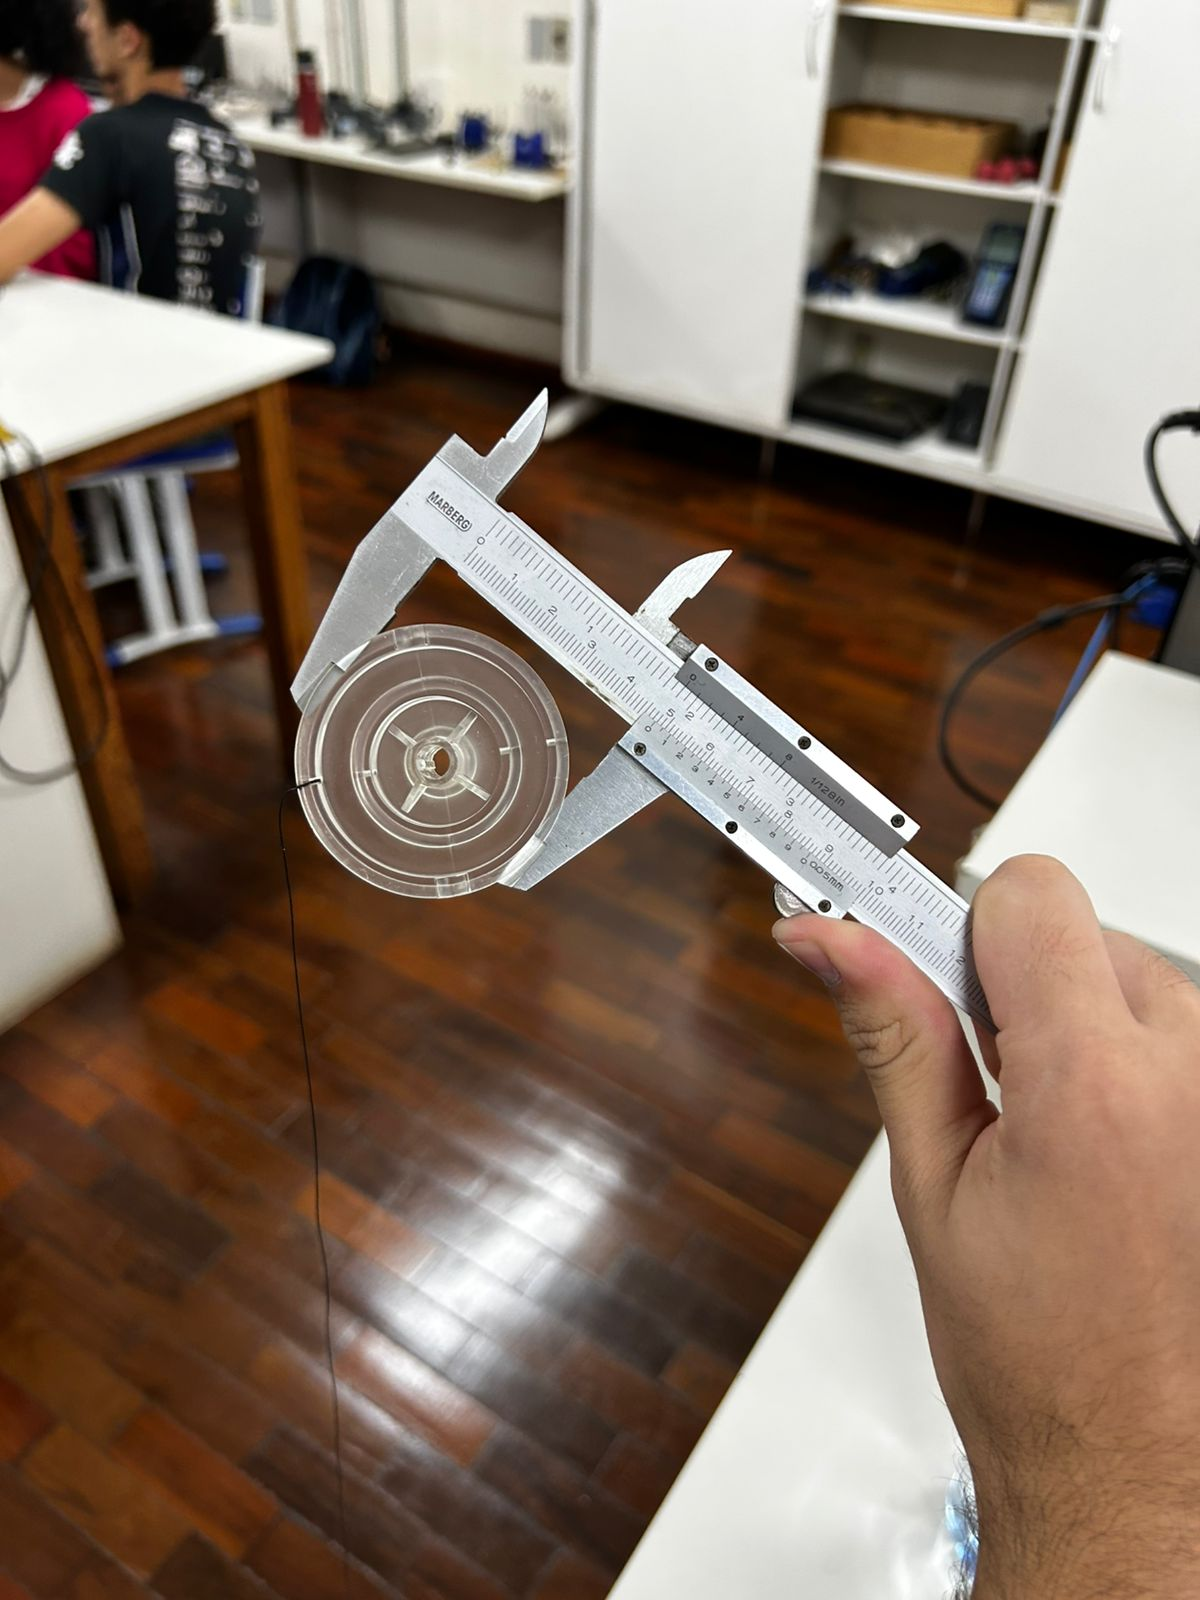
\includegraphics[width=0.4\textwidth]{media/photos/equipamentos/r1_diameter.png}
\caption{Medida do diâmetro da polia. Fonte: Autor}~\label{r1_diameter}
\end{figure}

\begin{figure}[H]
\centering
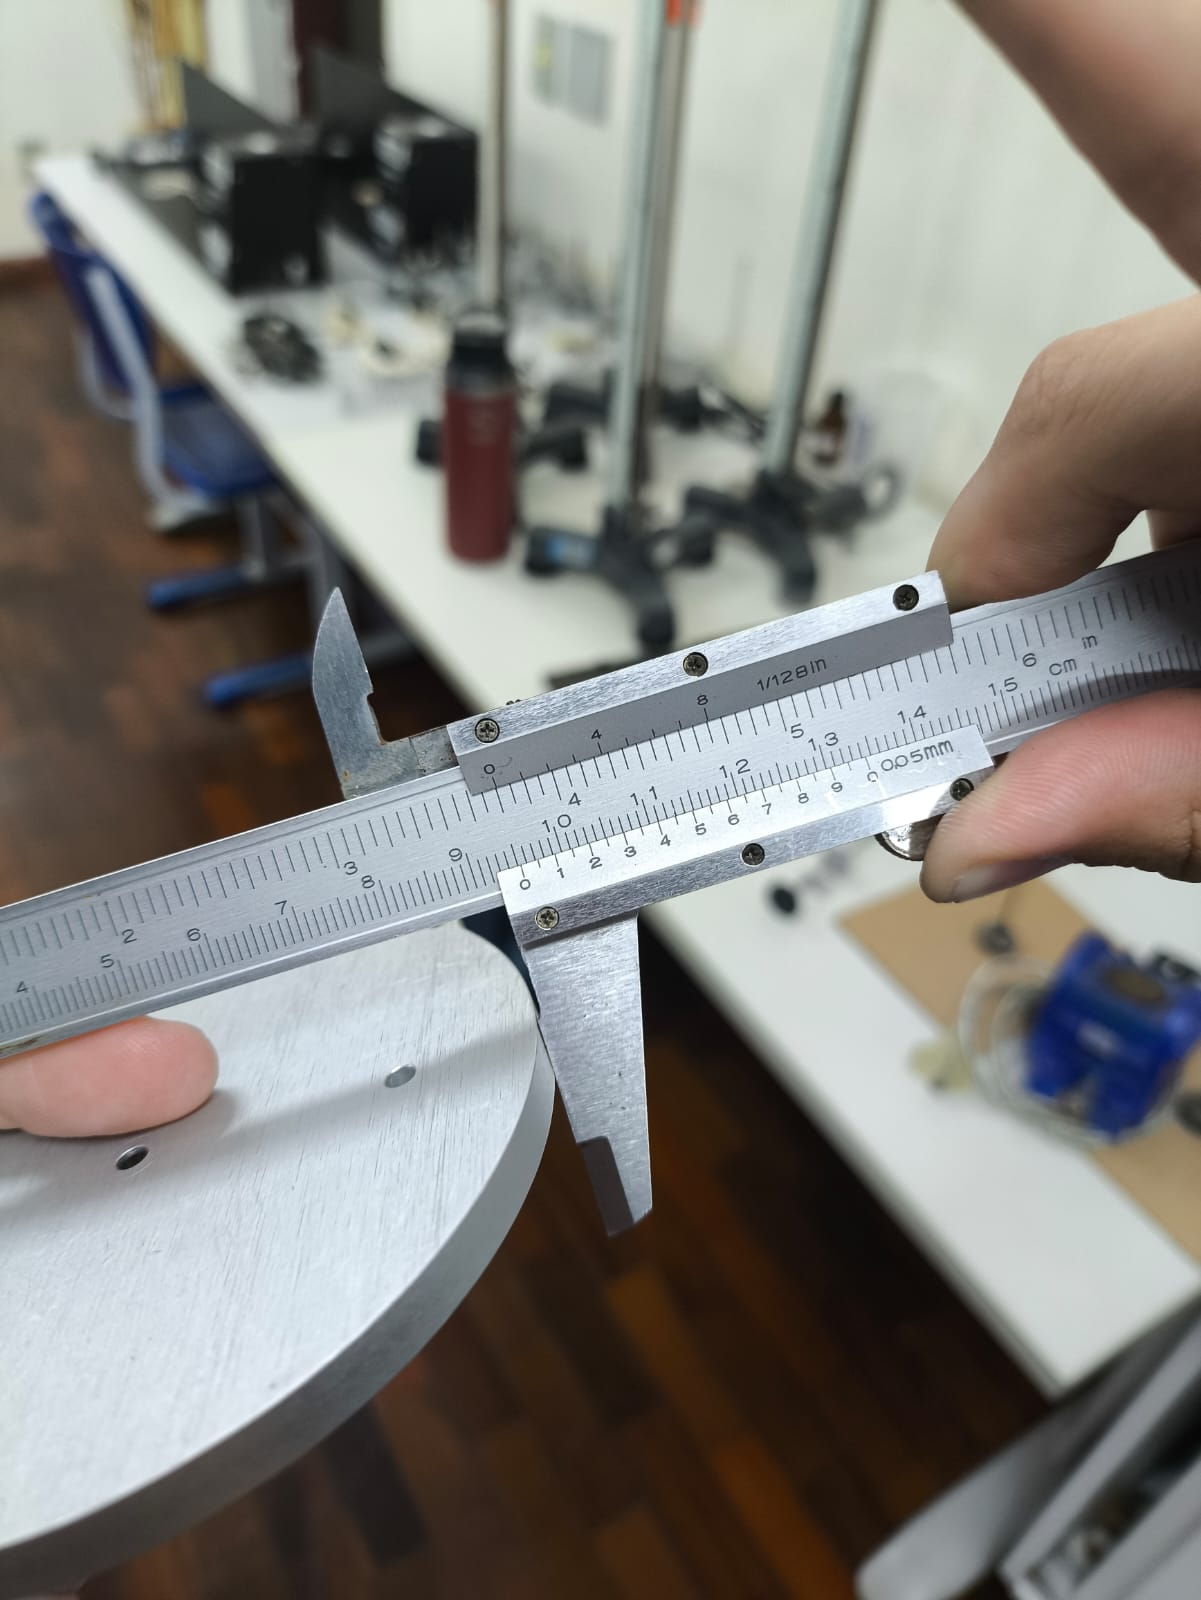
\includegraphics[width=0.4\textwidth]{media/photos/equipamentos/r2_diameter.png}
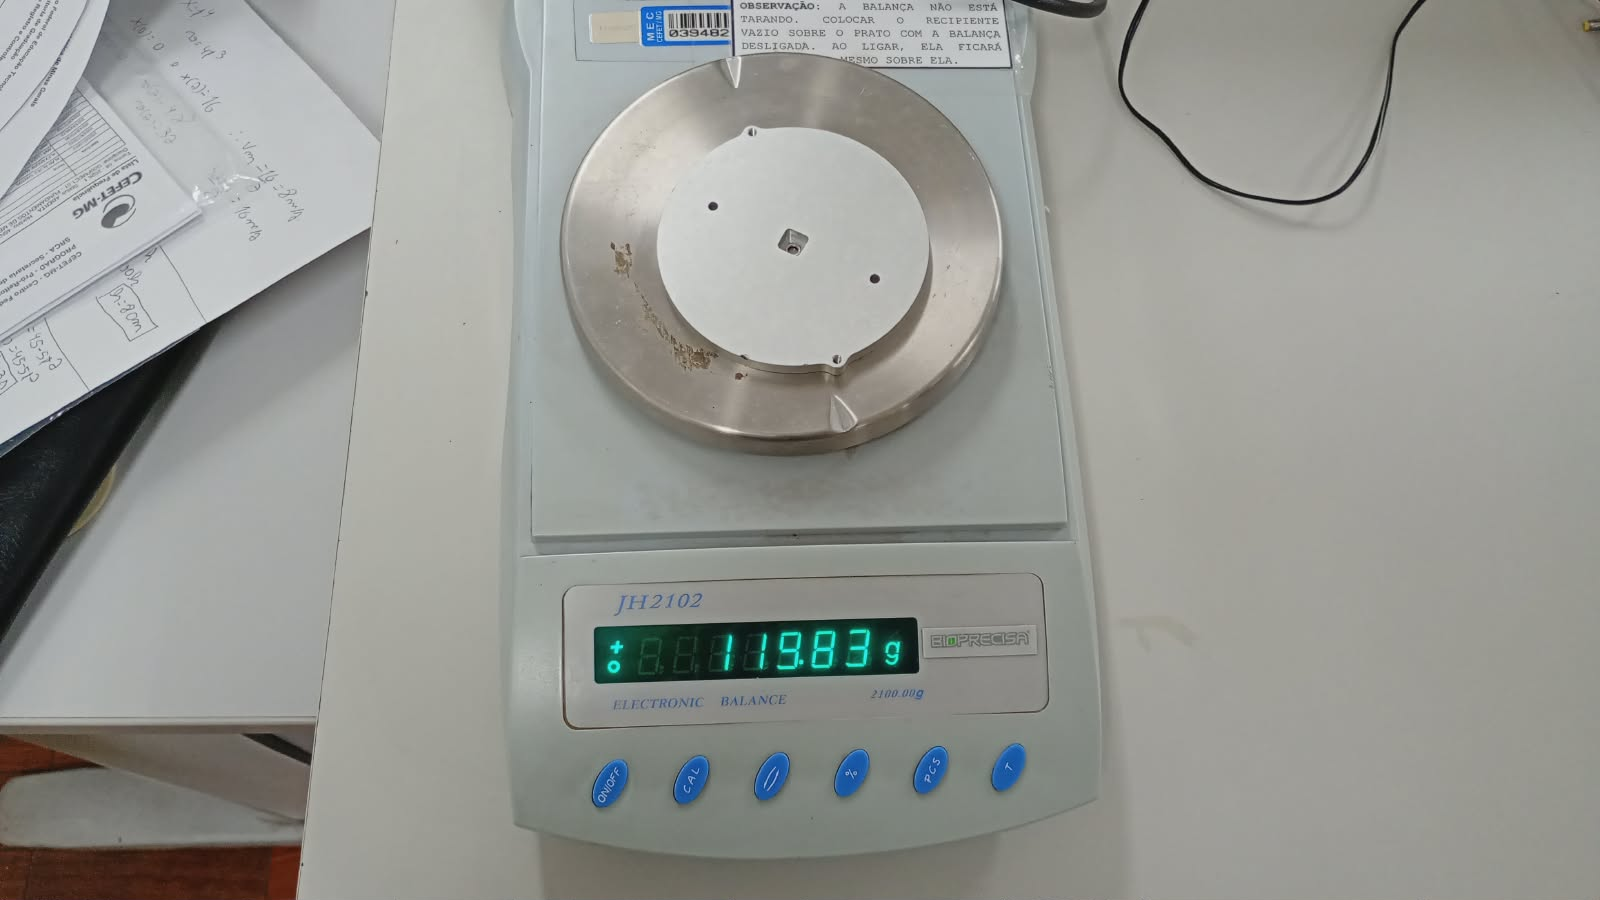
\includegraphics[width=0.8\textwidth]{media/photos/equipamentos/massa_2.png}
\caption{Dimensões do disco. Fonte: Autor}~\label{r2_diameter}
\end{figure}

\begin{figure}[H]
\centering
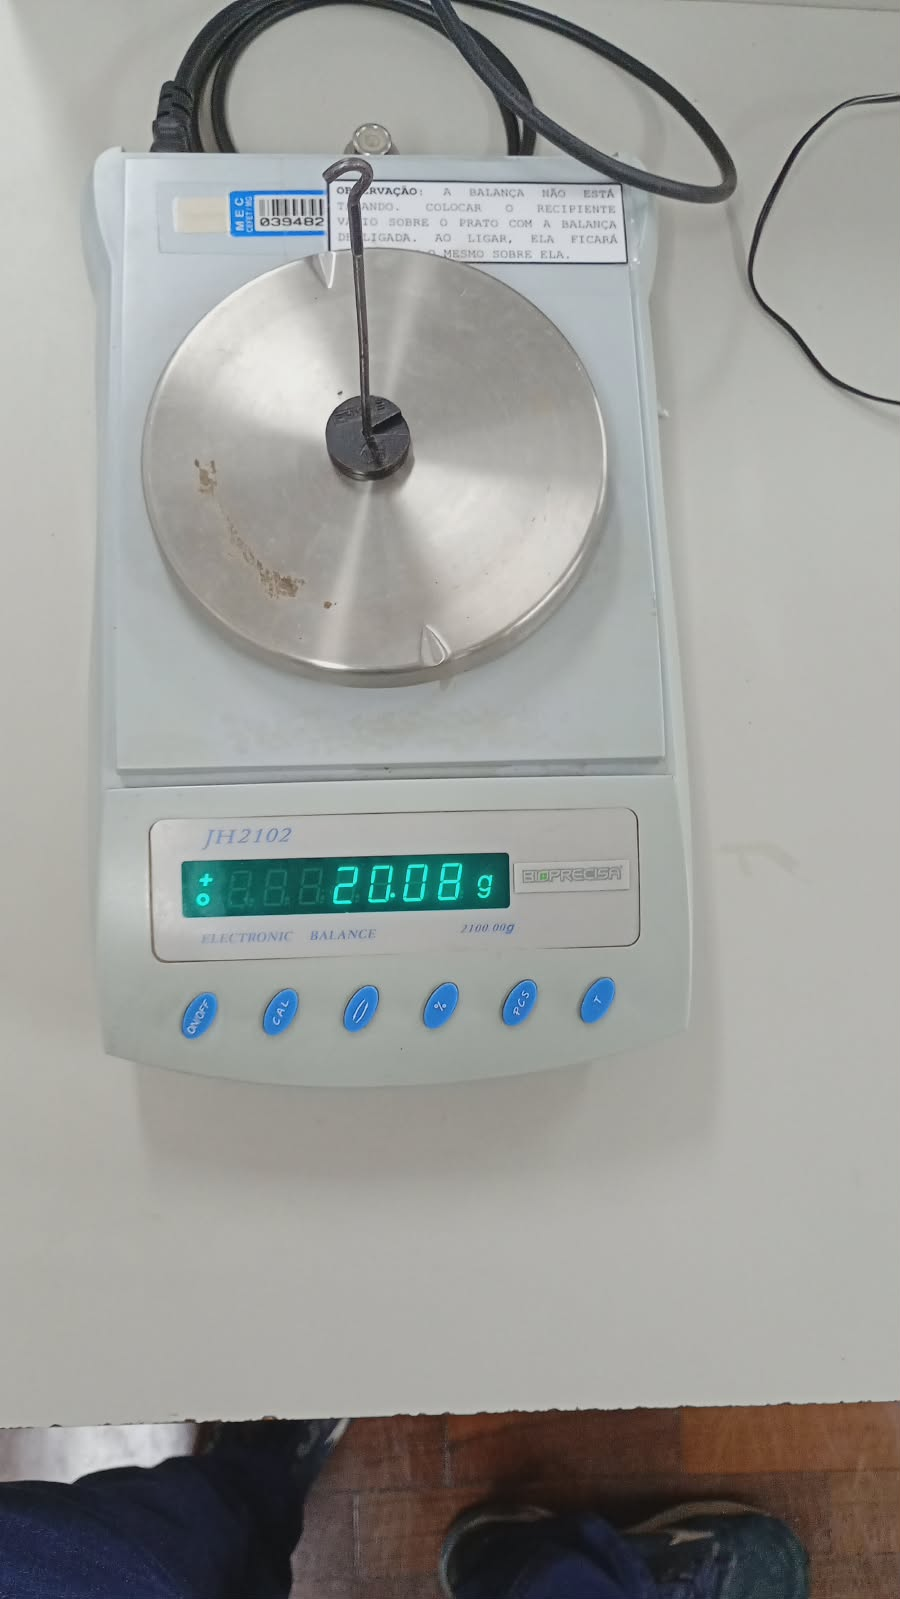
\includegraphics[width=0.4\textwidth]{media/photos/equipamentos/massa_3.png}
\caption{Medida da Massa Pendente. Fonte: Autor}~\label{massa_pendente}
\end{figure}

\subsubsection{Organização dos dados em tabela}
O Datalogger utilizado já salva os dados coletados em tabelas, mas alguns ajustes foram necessários para facilitar a análise. Foram feitos ajustes de formatação, e remoção de rúido. Os dados ajustados, removendo valores negativos e subtraindo o valor inicial para começar do tempo $t=0$ e posição angular $\theta=0$. Após isso foram organizados em tabelas para cada registro, facilitando a construção dos gráficos e a realização dos ajustes lineares no SciDAVis. 

\subsubsection{Construção de gráficos e realização de ajustes no SciDAVis}
Os dados organizados em tabela foram importados para o software SciDAVis para análise de dados. Gráficos de posição angular em função do tempo foram construídos, e ajustes lineares foram realizados para determinar o coeficiente $A$ do ajuste linear, que é utilizado para o cálculo do momento de inércia do sistema. Para fins de comparação dos resultados, os ajustes lineares foram realizados tanto para o caso geral, quanto para o caso partindo do repouso.


\subsubsection{Determinação do momento de inércia do sistema e da polia}
Foi utilizada a equação \eqref{eq:moment_inertia_disk} para determinar o momento de inércia do disco $I_{disco}$.

A partir dos coeficientes dos ajustes lineares calculados experimentalmente, 
foi possível determinar o momento de inércia do sistema $I_{total}$ utilizando a equação \eqref{eq:moment_inertia_final}. Com o momento de inércia do sistema $I_{total}$ e do disco $I_{disco}$, foi possível determinar o momento de inércia da polia $I_{polia}$ a partir da equação \eqref{eq:moment_inertia_polia}.

\section{Resultados e Discussão}

As dimensões do sistema encontradas foram:

\begin{itemize}
    \item Raio da polia $r_p$: $23,825 \times 10^{-3} \pm 0,005 \times 10^{-3}  \, m$;
    \item Raio do disco $r_{disco}$: $47,625\times 10^{-3} \pm 0,005 \times 10^{-3}  \, m$;
    \item Massa do disco $m_{disco}$: $119,3\times 10^{-3}  \, kg$;
    \item Massa pendente $m$: $20,08\times 10^{-3} \, kg$.
    \item Aceleração da gravidade em Belo Horizonte,  $g_{bh}$: $9,78 \, m/s^2$.
    \item Momento de inércia do disco $I_{disco}$: $\frac{1}{2} m_{disco} r_{disco}^2 = 1,3529 \times 10^{-4} \, kg m^2$.
\end{itemize}

\subsection{DataSets}

Os resultados brutos obtidos para a posição angular do disco em função do tempo para ambos conjuntos de dados foram organizados em tabelas, e depois filtrados e ajustados para facilitar a análise. As tabelas com os dados brutos e ajustados de posição angular em função do tempo para ambos conjuntos de dados estão apresentadas a seguir.

\subsubsection{DataSet 1}

\begin{longtable}{
    S[table-format=1.4] S[table-format=3.3] | % Bloco 1
    S[table-format=1.4] S[table-format=3.3] | % Bloco 2
    S[table-format=1.4] S[table-format=3.3]   % Bloco 3
}
\caption{Dados Brutos experimentais de posição angular em função do tempo para o Conjunto de Dados 1.}
\label{tab:dados_cinematicos_1_raw} \\

\toprule
% Cabeçalho da PRIMEIRA página
\multicolumn{1}{c}{\textbf{Tempo (s)}} & \multicolumn{1}{c|}{\textbf{Posição (rad)}} &
\multicolumn{1}{c}{\textbf{Tempo (s)}} & \multicolumn{1}{c|}{\textbf{Posição (rad)}} &
\multicolumn{1}{c}{\textbf{Tempo (s)}} & \multicolumn{1}{c}{\textbf{Posição (rad)}} \\
\midrule
\endfirsthead

% Cabeçalho que vai se repetir nas PRÓXIMAS páginas
\multicolumn{6}{c}{{\tablename\ \thetable{} -- continuação da página anterior}} \\
\toprule
\multicolumn{1}{c}{\textbf{Tempo (s)}} & \multicolumn{1}{c|}{\textbf{Posição (rad)}} &
\multicolumn{1}{c}{\textbf{Tempo (s)}} & \multicolumn{1}{c|}{\textbf{Posição (rad)}} &
\multicolumn{1}{c}{\textbf{Tempo (s)}} & \multicolumn{1}{c}{\textbf{Posição (rad)}} \\
\midrule
\endhead

% Rodapé provisório no fim de cada página
\midrule
\multicolumn{6}{r}{{\footnotesize \textit{Continua na próxima página...}}} \\
\endfoot

% Rodapé definitivo no fim da tabela inteira
\bottomrule
\endlastfoot

0,0000  &   0,438 &     0,0100  &   0,511 &     0,0200  &   0,586 \\
0,0300  &   0,666 &     0,0400  &   0,748 &     0,0500  &   0,834 \\
0,0600  &   0,922 &     0,0700  &   1,015 &     0,0800  &   1,109 \\
0,0900  &   1,206 &     0,1000  &   1,308 &     0,1100  &   1,412 \\
0,1200  &   1,519 &     0,1300  &   1,629 &     0,1400  &   1,744 \\
0,1500  &   1,860 &     0,1600  &   1,979 &     0,1700  &   2,102 \\
0,1800  &   2,226 &     0,1900  &   2,355 &     0,2000  &   2,487 \\
0,2100  &   2,620 &     0,2200  &   2,758 &     0,2300  &   2,900 \\
0,2300  &   2,900 &     0,2400  &   3,043 &     0,2500  &   3,189 \\
0,2600  &   3,340 &     0,2700  &   3,492 &     0,2800  &   3,646 \\
0,2900  &   3,804 &     0,3000  &   3,965 &     0,3100  &   4,130 \\
0,3200  &   4,296 &     0,3300  &   4,464 &     0,3400  &   4,639 \\
0,3500  &   4,814 &     0,3600  &   4,992 &     0,3700  &   5,174 \\
0,3800  &   5,360 &     0,3900  &   5,548 &     0,4000  &   5,740 \\
0,4100  &   5,934 &     0,4200  &   6,131 &     0,4300  &   6,332 \\
0,4400  &   6,536 &     0,4500  &   6,743 &     0,4600  &   6,954 \\
0,4700  &   7,168 &     0,4800  &   7,383 &     0,4900  &   7,603 \\
0,5000  &   7,826 &     0,5100  &   8,052 &     0,5200  &   8,280 \\
0,5300  &   8,512 &     0,5400  &   8,746 &     0,5500  &   8,983 \\
0,5600  &   9,224 &     0,5700  &   9,467 &     0,5800  &   9,714 \\
0,5900  &   9,964 &     0,6000  &   10,216 &    0,6100  &   10,473 \\
0,6200  &   10,732 &    0,6300  &   10,994 &    0,6400  &   11,259 \\
0,6500  &   11,527 &    0,6600  &   11,798  &   0,6700  &   12,072  \\
0,6800  &   12,350  &   0,6900  &   12,629  &   0,7000  &   12,912  \\
0,7100  &   13,199  &   0,7200  &   13,490  &   0,7300  &   13,782  \\
0,7400  &   14,077  &   0,7500  &   14,378  &   0,7600  &   14,681  \\
0,7700  &   14,985  &   0,7800  &   15,293  &   0,7900  &   15,604  \\
0,8000  &   15,918  &   0,8100  &   16,236  &   0,8200  &   16,556  \\
0,8300  &   16,880  &   0,8400  &   17,207  &   0,8500  &   17,536  \\
0,8600  &   17,868  &   0,8700  &   18,202  &   0,8800  &   18,542  \\
0,8900  &   18,883  &   0,9000  &   19,227  &   0,9100  &   19,574  \\
0,9200  &   19,924  &   0,9300  &   20,279  &   0,9400  &   20,636  \\
0,9500  &   20,995  &   0,9600  &   21,358  &   0,9700  &   21,724  \\
0,9800  &   22,093  &   0,9900  &   22,466  &   1,0000  &   22,841  \\
1,0100  &   23,220  &   1,0200  &   23,601  &   1,0300  &   23,984  \\
1,0400  &   24,372  &   1,0500  &   24,762  &   1,0600  &   25,155  \\
1,0700  &   25,551  &   1,0800  &   25,951  &   1,0900  &   26,353  \\
1,1000  &   26,759  &   1,1100  &   27,167  &   1,1200  &   27,578  \\
1,1300  &   27,993  &   1,1400  &   28,411  &   1,1500  &   28,832  \\
1,1600  &   29,255  &   1,1700  &   29,682  &   1,1800  &   30,112  \\
1,1900  &   30,544  &   1,2000  &   30,978  &   1,2100  &   31,408  \\
1,2200  &   31,840  &   1,2300  &   32,274  &   1,2400  &   32,706  \\
1,2500  &   33,138  &   1,2600  &   33,570  &   1,2700  &   34,001  \\
1,2800  &   34,433  &   1,2900  &   34,865  &   1,3000  &   35,297  \\
1,3100  &   35,729  &   1,3200  &   36,161  &   1,3300  &   36,593  \\
1,3400  &   37,024  &   1,3500  &   37,454  &   1,3600  &   37,886  \\
1,3700  &   38,316  &   1,3800  &   38,747  &   1,3900  &   39,176  \\
1,4000  &   39,606  &   1,4100  &   40,024  &   1,4200  &   40,439  \\
1,4300  &   40,841  &   1,4400  &   41,215  &   1,4500  &   41,560  \\
1,4600  &   41,884  &   1,4700  &   42,170  &   1,4800  &   42,407  \\
1,4900  &   42,595  &   1,5000  &   42,735  &   1,5100  &   42,836  \\
1,5200  &   42,906  &   1,5300  &   42,953  &   1,5400  &   42,988  \\
1,5500  &   43,015  &   1,5600  &   43,034  &   1,5700  &   43,043  \\

\end{longtable}

\begin{longtable}{
    S[table-format=1.4] S[table-format=3.3] | % Bloco 1
    S[table-format=1.4] S[table-format=3.3] | % Bloco 2
    S[table-format=1.4] S[table-format=3.3]   % Bloco 3
}
\caption{Dados Filtrados experimentais de posição angular em função do tempo para o Conjunto de Dados 1.}
\label{tab:dados_cinematicos_1_filtered} \\

\toprule
% Cabeçalho da PRIMEIRA página
\multicolumn{1}{c}{\textbf{Tempo (s)}} & \multicolumn{1}{c|}{\textbf{Posição (rad)}} &
\multicolumn{1}{c}{\textbf{Tempo (s)}} & \multicolumn{1}{c|}{\textbf{Posição (rad)}} &
\multicolumn{1}{c}{\textbf{Tempo (s)}} & \multicolumn{1}{c}{\textbf{Posição (rad)}} \\
\midrule
\endfirsthead

% Cabeçalho que vai se repetir nas PRÓXIMAS páginas
\multicolumn{6}{c}{{\tablename\ \thetable{} -- continuação da página anterior}} \\
\toprule
\multicolumn{1}{c}{\textbf{Tempo (s)}} & \multicolumn{1}{c|}{\textbf{Posição (rad)}} &
\multicolumn{1}{c}{\textbf{Tempo (s)}} & \multicolumn{1}{c|}{\textbf{Posição (rad)}} &
\multicolumn{1}{c}{\textbf{Tempo (s)}} & \multicolumn{1}{c}{\textbf{Posição (rad)}} \\
\midrule
\endhead

% Rodapé provisório no fim de cada página
\midrule
\multicolumn{6}{r}{{\footnotesize \textit{Continua na próxima página...}}} \\
\endfoot

% Rodapé definitivo no fim da tabela inteira
\bottomrule
\endlastfoot
0,0000  &   0,000 &     0,0100  &   0,073 &     0,0200  &   0,148 \\
0,0300  &   0,228 &     0,0400  &   0,310 &     0,0500  &   0,396 \\
0,0600  &   0,484 &     0,0700  &   0,577 &     0,0800  &   0,671 \\
0,0900  &   0,768 &     0,1000  &   0,870 &     0,1100  &   0,974 \\
0,1200  &   1,081 &     0,1300  &   1,191 &     0,1400  &   1,306 \\
0,1500  &   1,422 &     0,1600  &   1,541 &     0,1700  &   1,664 \\
0,1800  &   1,788 &     0,1900  &   1,917 &     0,2000  &   2,049 \\
0,2100  &   2,182 &     0,2200  &   2,320 &     0,2300  &   2,462 \\
0,2400  &   2,605 &     0,2500  &   2,751 &     0,2600  &   2,902 \\
0,2700  &   3,054 &     0,2800  &   3,208 &     0,2900  &   3,366 \\
0,3000  &   3,527 &     0,3100  &   3,692 &     0,3200  &   3,858 \\
0,3300  &   4,026 &     0,3400  &   4,201 &     0,3500  &   4,376 \\
0,3600  &   4,554 &     0,3700  &   4,736 &     0,3800  &   4,922 \\
0,3900  &   5,110 &     0,4000  &   5,302 &     0,4100  &   5,496 \\
0,4200  &   5,693 &     0,4300  &   5,894 &     0,4400  &   6,098 \\
0,4500  &   6,305 &     0,4600  &   6,516 &     0,4700  &   6,730 \\
0,4800  &   6,945 &     0,4900  &   7,165 &     0,5000  &   7,388 \\
0,5100  &   7,614 &     0,5200  &   7,842 &     0,5300  &   8,074 \\
0,5400  &   8,308 &     0,5500  &   8,545 &     0,5600  &   8,786 \\
0,5700  &   9,029 &     0,5800  &   9,276 &     0,5900  &   9,526 \\
0,6000  &   9,778 &     0,6100  &   10,035 &   0,6200  &   10,294 \\
0,6300  &   10,556 &    0,6400  &   10,821 &   0,6500  &   11,089 \\
0,6600  &   11,360 &    0,6700  &   11,634 &   0,6800  &   11,912 \\
0,6900  &   12,191 &    0,7000  &   12,474 &   0,7100  &   12,761 \\
0,7200  &   13,052 &    0,7300  &   13,344 &   0,7400  &   13,639 \\
0,7500  &   13,940 &    0,7600  &   14,243 &   0,7700  &   14,547 \\
0,7800  &   14,855 &    0,7900  &   15,166 &   0,8000  &   15,480 \\
0,8100  &   15,798 &    0,8200  &   16,118 &   0,8300  &   16,442 \\
0,8400  &   16,769 &    0,8500  &   17,098 &   0,8600  &   17,430 \\
0,8700  &   17,764 &    0,8800  &   18,104 &   0,8900  &   18,445 \\
0,9000  &   18,789 &    0,9100  &   19,136 &   0,9200  &   19,486 \\
0,9300  &   19,841 &    0,9400  &   20,198 &   0,9500  &   20,557 \\
0,9600  &   20,920 &    0,9700  &   21,286 &   0,9800  &   21,655 \\
0,9900  &   22,028 &    1,0000  &   22,403 &   1,0100  &   22,782 \\
0,0200  &   23,163 &    1,0300  &   23,546 &   1,0400  &   23,934 \\
0,0500  &   24,324 &    1,0600  &   24,717 &   1,0700  &   25,113 \\
0,0800  &   25,513 &    1,0900  &   25,915 &   1,1000  &   26,321 \\
0,1100  &   26,729 &    1,1200  &   27,140 &   1,1300  &   27,555 \\
0,1400  &   27,973 &    1,1500  &   28,394 &   1,1600  &   28,817 \\
0,1700  &   29,244 &    1,1800  &   29,674 &   1,1900  &   30,106 \\
0,2000  &   30,540 &    1,2100  &   30,970 &   1,2200  &   31,402 \\
0,2300  &   31,836 &    1,2400  &   32,268 &   1,2500  &   32,700 \\
0,2600  &   33,132 &    1,2700  &   33,563 &   1,2800  &   33,995 \\
0,2900  &   34,427 &    1,3000  &   34,859 &   1,3100  &   35,291 \\
0,3200  &   35,723 &    1,3300  &   36,155 &   1,3400  &   36,586 \\
0,3500  &   37,016 &    1,3600  &   37,448 &   1,3700  &   37,878 \\
0,3800  &   38,309 &    1,3900  &   38,738 &   1,4000  &   39,168 \\
0,4100  &   39,586 &    1,4200  &   40,001 &   1,4300  &   40,403 \\  

\end{longtable}

\subsubsection{DataSet 2}

\begin{table}[H]
\centering
\caption{Dados Brutos experimentais de posição angular em função do tempo para o Conjunto de Dados 2.}
\label{tab:dados_cinematicos_2_raw}
\resizebox{\textwidth}{!}{
\begin{tabular}{
    S[table-format=1.4] S[table-format=3.3] | % Bloco 1
    S[table-format=1.4] S[table-format=3.3] | % Bloco 2
    S[table-format=1.4] S[table-format=3.3]   % Bloco 3
}
\toprule
\multicolumn{1}{c}{\textbf{Tempo (s)}} & \multicolumn{1}{c|}{\textbf{Posição (rad)}} &
\multicolumn{1}{c}{\textbf{Tempo (s)}} & \multicolumn{1}{c|}{\textbf{Posição (rad)}} &
\multicolumn{1}{c}{\textbf{Tempo (s)}} & \multicolumn{1}{c}{\textbf{Posição (rad)}} \\
\midrule

0,0000  & 0,000     & 0,0200    & 0,000     & 0,0400    & -0,002    \\
0,0600  & -0,002    & 0,0800    & -0,002    & 0,1000    & -0,002    \\
0,1200  & -0,002    & 0,1400    & -0,002    & 0,1600    & 0,003     \\
0,1800  & 0,014     & 0,2000    & 0,031     & 0,2200    & 0,066     \\
0,2400  & 0,110     & 0,2600    & 0,170     & 0,2800    & 0,240     \\
0,3000  & 0,324     & 0,3200    & 0,421     & 0,3400    & 0,528     \\
0,3600  & 0,649     & 0,3800    & 0,782     & 0,4000    & 0,925     \\
0,4200  & 1,081     & 0,4400    & 1,249     & 0,4600    & 1,428     \\
0,4800  & 1,619     & 0,5000    & 1,824     & 0,5200    & 2,034     \\
0,5400  & 2,257     & 0,5600    & 2,496     & 0,5800    & 2,738     \\
0,6000  & 2,997     & 0,6200    & 3,264     & 0,6400    & 3,537     \\
0,6600  & 3,830     & 0,6800    & 4,123     & 0,7000    & 4,433     \\
0,7200  & 4,752     & 0,7400    & 5,083     & 0,7600    & 5,426     \\
0,7800  & 5,784     & 0,8000    & 6,143     & 0,8200    & 6,519     \\
0,8400  & 6,913     & 0,8600    & 7,306     & 0,8800    & 7,717     \\
0,9000  & 8,146     & 0,9200    & 8,575     & 0,9400    & 9,020     \\
0,9600  & 9,478     & 0,9800    & 9,946     & 1,0000    & 10,429    \\
1,0200  & 10,928    & 1,0400    & 11,426    & 1,0600    & 11,943    \\
1,0800  & 12,480    & 1,1000    & 13,012    & 1,1200    & 13,575    \\
1,1400  & 14,142    & 1,1600    & 14,712    & 1,1800    & 15,311    \\
1,2000  & 15,904    & 1,2200    & 16,519    & 1,2400    & 17,155    \\
1,2600  & 17,783    & 1,2800    & 18,433    & 1,3000    & 19,106    \\
1,3200  & 19,768    & 1,3400    & 20,455    & 1,3600    & 21,163    \\
1,3800  & 21,861    & 1,4000    & 22,583    & 1,4200    & 23,317    \\
1,4400  & 24,063    & 1,4600    & 24,820    & 1,4800    & 25,602    \\
1,5000  & 26,372    & 1,5200    & 27,167    & 1,5400    & 27,973    \\
1,5600  & 28,791    & 1,5800    & 29,635    & 1,6000    & 30,478    \\
1,6200  & 31,312    & 1,6400    & 32,157    & 1,6600    & 33,017    \\
1,6800  & 33,848    & 1,7000    & 34,707    & 1,7200    & 35,552    \\
1,7400  & 36,383    & 1,7600    & 37,240    & 1,7800    & 38,084    \\
1,8000  & 38,915    & 1,8200    & 39,769    & 1,8400    & 40,599    \\
1,8600  & 41,441    &     &      & 	    &      \\

\bottomrule
\end{tabular}
}
\end{table}

\begin{table}[H]
\centering
\caption{Dados Filtrados experimentais de posição angular em função do tempo para o Conjunto de Dados 2.}
\label{tab:dados_cinematicos_2_filtered}
\resizebox{\textwidth}{!}{
\begin{tabular}{
    S[table-format=1.4] S[table-format=3.3] | % Bloco 1
    S[table-format=1.4] S[table-format=3.3] | % Bloco 2
    S[table-format=1.4] S[table-format=3.3]   % Bloco 3
}
\toprule
\multicolumn{1}{c}{\textbf{Tempo (s)}} & \multicolumn{1}{c|}{\textbf{Posição (rad)}} &
\multicolumn{1}{c}{\textbf{Tempo (s)}} & \multicolumn{1}{c|}{\textbf{Posição (rad)}} &
\multicolumn{1}{c}{\textbf{Tempo (s)}} & \multicolumn{1}{c}{\textbf{Posição (rad)}} \\
\midrule

0,0000  &   0,000 &     0,0200  &   0,011 &     0,0400  &   0,028 \\
0,0600  &   0,063 &     0,0800  &   0,107 &     0,1000  &   0,167 \\
0,1200  &   0,237 &     0,1400  &   0,321 &     0,1600  &   0,418 \\
0,1800  &   0,525 &     0,2000  &   0,646 &     0,2200  &   0,779 \\
0,2400  &   0,922 &     0,2600  &   1,078 &     0,2800  &   1,246 \\
0,3000  &   1,425 &     0,3200  &   1,616 &     0,3400  &   1,821 \\
0,3600  &   2,031 &     0,3800  &   2,254 &     0,4000  &   2,493 \\
0,4200  &   2,735 &     0,4400  &   2,994 &     0,4600  &   3,261 \\
0,4800  &   3,534 &     0,5000  &   3,827 &     0,5200  &   4,120 \\
0,5400  &   4,430 &     0,5600  &   4,749 &     0,5800  &   5,080 \\
0,6000  &   5,423 &     0,6200  &   5,781 &     0,6400  &   6,140 \\
0,6600  &   6,516 &     0,6800  &   6,910 &     0,7000  &   7,303 \\
0,7200  &   7,714 &     0,7400  &   8,143 &     0,7600  &   8,572 \\
0,7800  &   9,017 &     0,8000  &   9,475 &     0,8200  &   9,943 \\
0,8400  &   10,426 &    0,8600  &   10,925 &    0,8800  &   11,423 \\
0,9000  &   11,940 &    0,9200  &   12,477 &    0,9400  &   13,009 \\
0,9600  &   13,572 &    0,9800  &   14,139 &    1,0000  &   14,709 \\
1,0200  &   15,308 &    1,0400  &   15,901 &    1,0600  &   16,516 \\
1,0800  &   17,152 &    1,1000  &   17,780 &    1,1200  &   18,430 \\
1,1400  &   19,103 &    1,1600  &   19,765 &    1,1800  &   20,452 \\
1,2000  &   21,160 &    1,2200  &   21,858 &    1,2400  &   22,580 \\
1,2600  &   23,314 &    1,2800  &   24,060 &    1,3000  &   24,817 \\
1,3200  &   25,599 &    1,3400  &   26,369 &    1,3600  &   27,164 \\
1,3800  &   27,970 &    1,4000  &   28,788 &    1,4200  &   29,632 \\
1,4400  &   30,475 &    1,4600  &   31,309 &    1,4800  &   32,154 \\
1,5000  &   33,014 &    1,5200  &   33,845 &    1,5400  &   34,704 \\
1,5600  &   35,549 &    1,5800  &   36,380 &    1,6000  &   37,237 \\
1,6200  &   38,081 &    1,6400  &   38,912 &    1,6600  &   39,766 \\
1,6800  &   40,596 &    1,7000  &   41,438 &            &          \\

\bottomrule
\end{tabular}
}
\end{table}

\subsection{Ajustes Lineares}

Após a filtragem dos dados, foram realizados ajustes lineares para os casos partindo do repouso e para o caso geral, utilizando as equações \eqref{eq:angular_position_repouso} e \eqref{eq:angular_position_geral}, respectivamente.

\subsubsection{Ajuste Linear para o caso a partir do Repouso para o Dataset 1}

\begin{figure}[H]
\centering
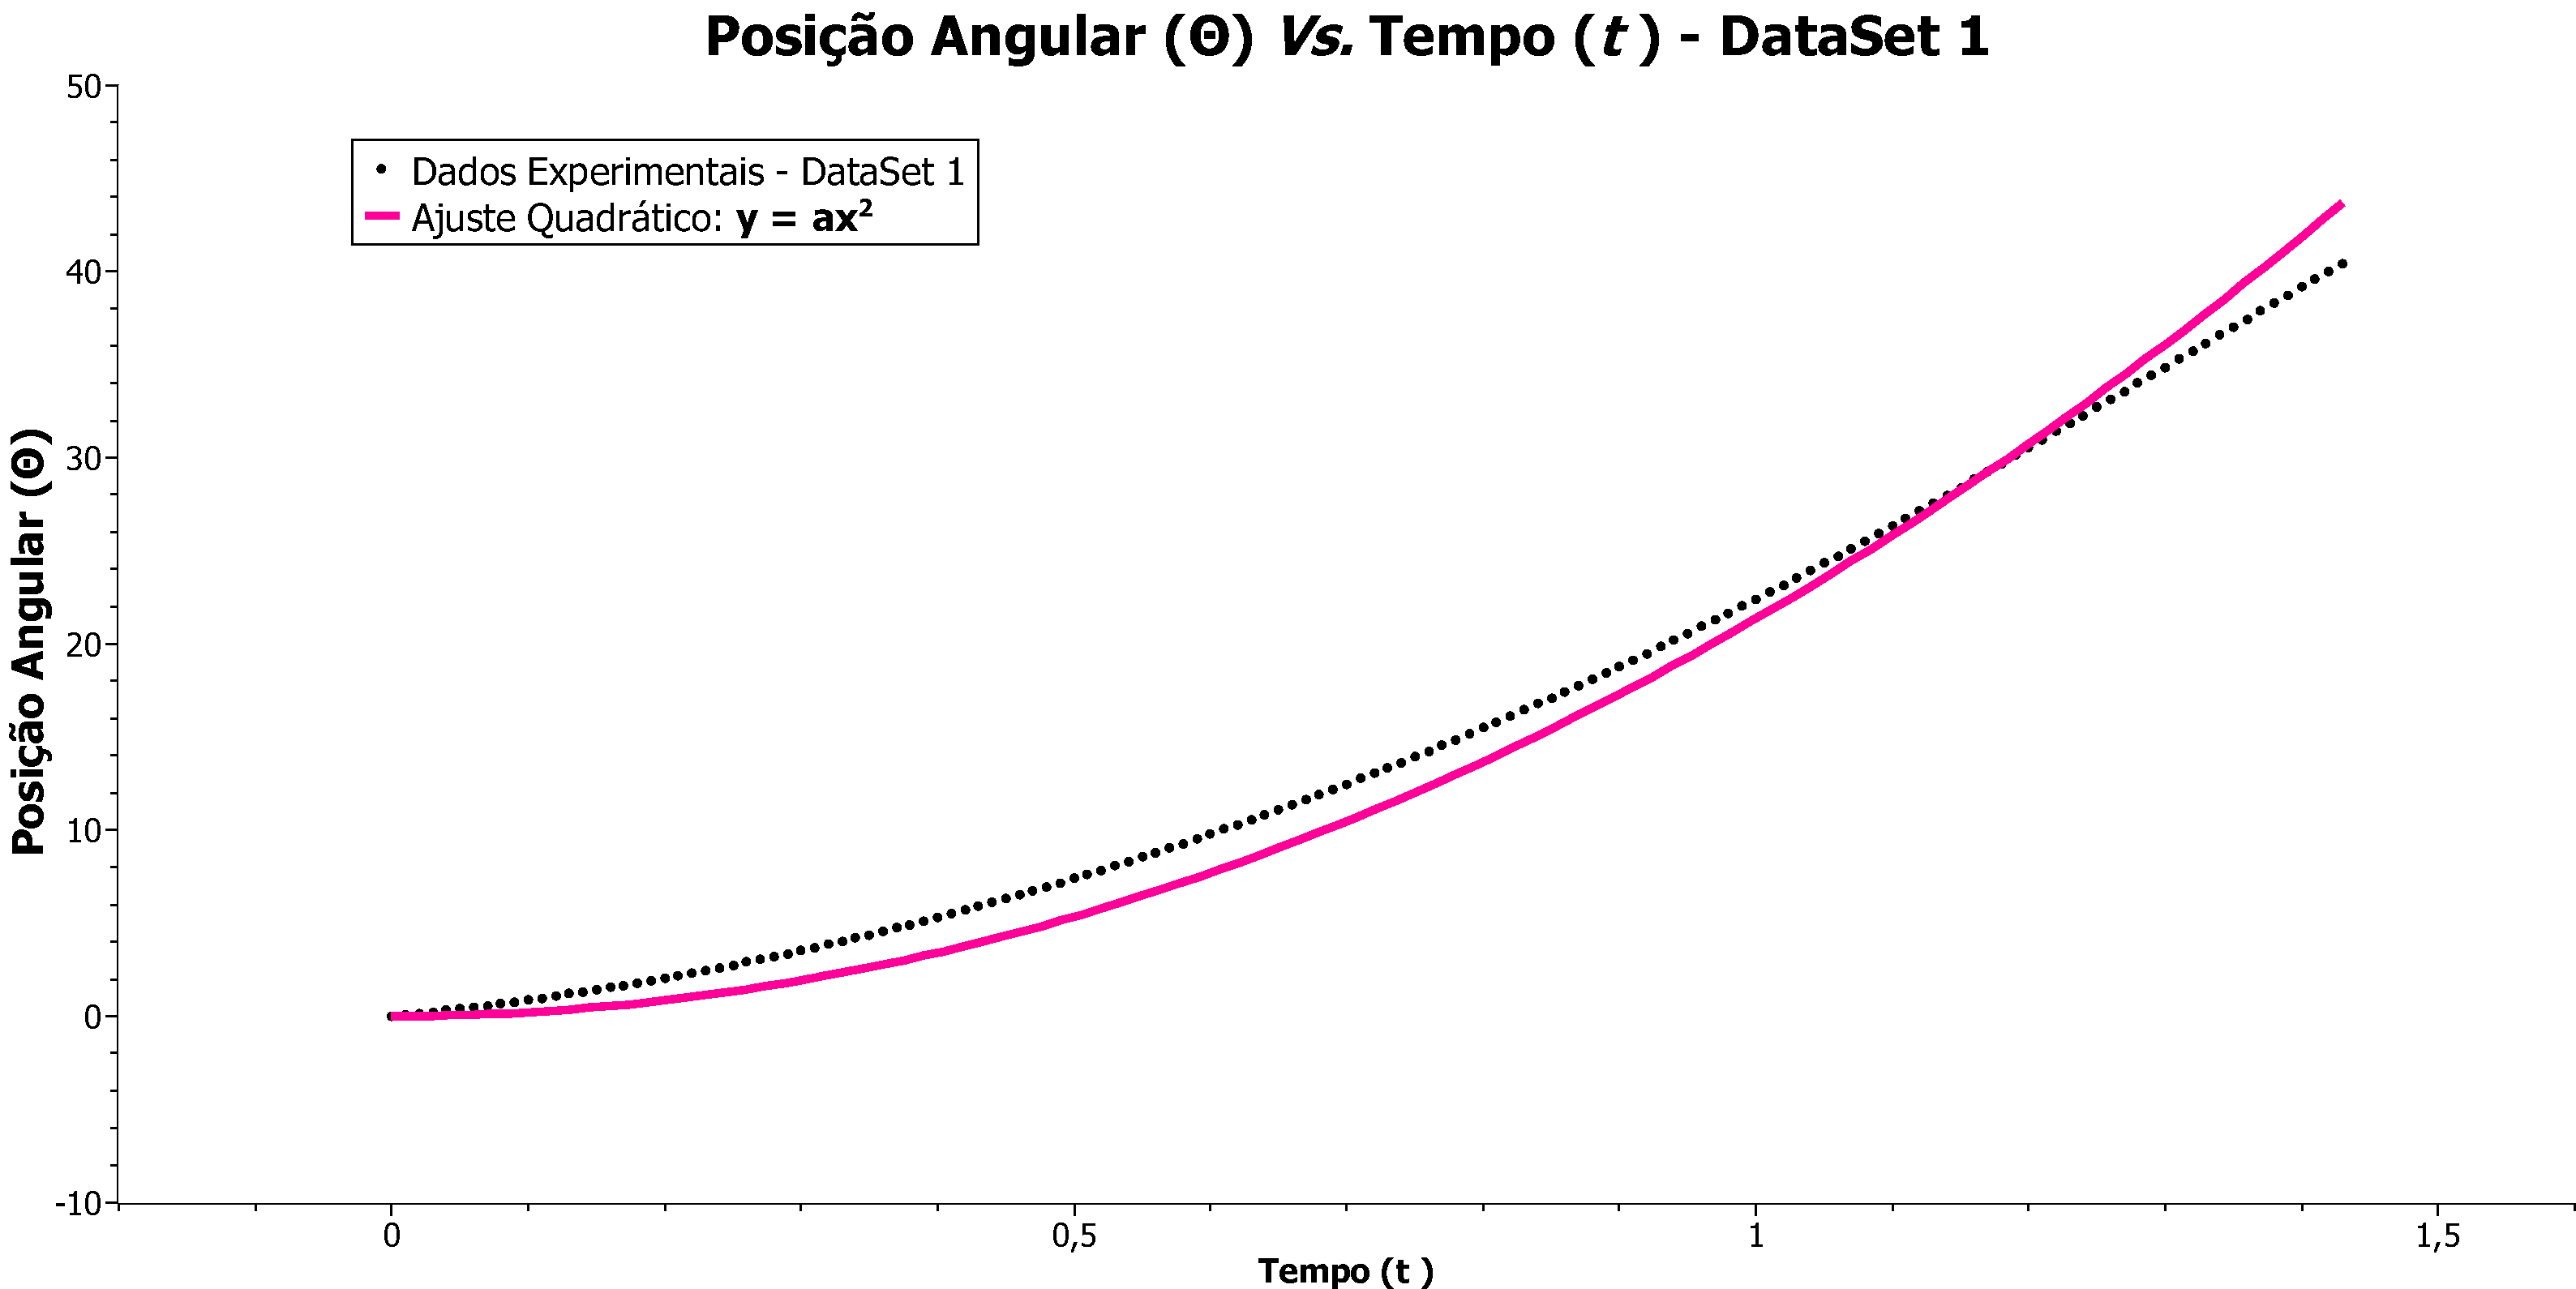
\includegraphics[width=0.9\textwidth]{media/graphs/r1_dataset1}
\caption{Ajuste Linear para o Caso a partir do Repouso - Dataset 1. Fonte: Autor}~\label{fig:ajuste_linear_r1_dataset1}
\end{figure}

O ajuste linear para o caso partindo do repouso resultou no coeficiente $A_{r1} = 21,3 \pm 0,1$.

\subsubsection{Log do SciDAVis}
\begin{verbatim}
[sábado, 18 de abril de 2026 12:03:54 Hora oficial do Brasil	Plot: ''Graph1'']
Non-linear fit of dataset: Table2_Angular Position, using function: a*x^2
Y standard errors: Unknown
Scaled Levenberg-Marquardt algorithm with tolerance = 0,0001
From x = 0 to x = 1,43
a  = 21,3501925593388 +/- 0,141943189091119
--------------------------------------------------------------------------------------
Chi^2 = 350,620380284854
R^2 = 0,993719051183645
---------------------------------------------------------------------------------------
Iterations = 1
Status = success
---------------------------------------------------------------------------------------
\end{verbatim}

\subsubsection{Ajuste Linear Geral para o Dataset 1}

\begin{figure}[H]
\centering
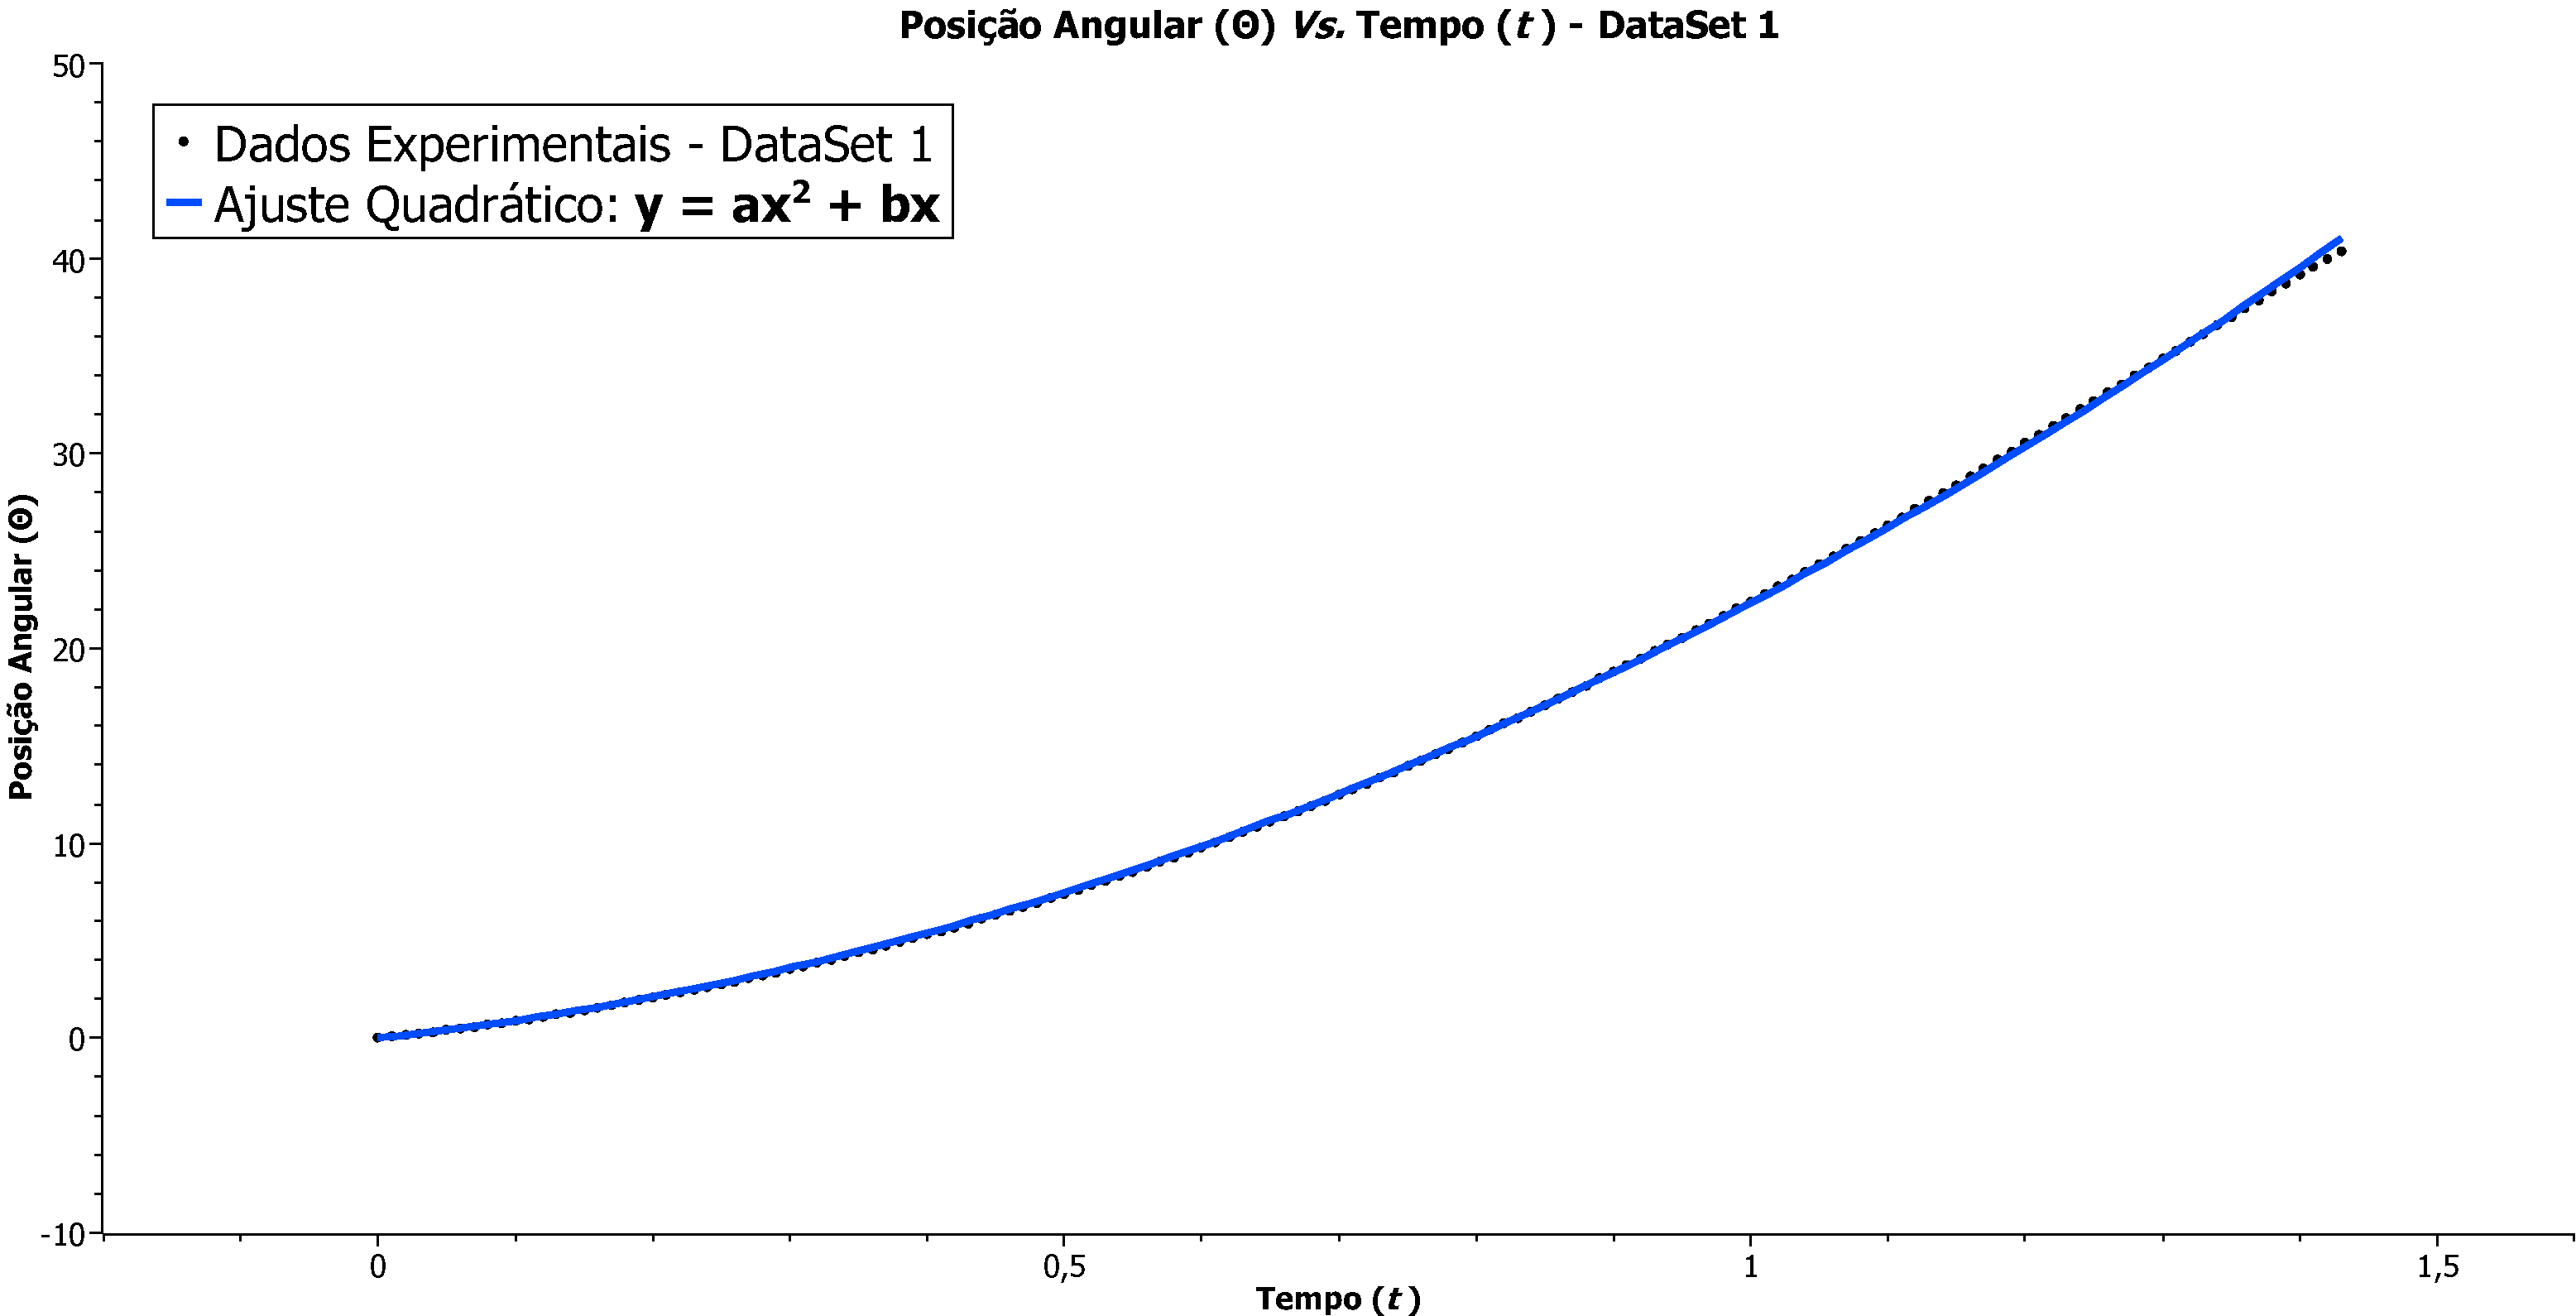
\includegraphics[width=0.9\textwidth]{media/graphs/g1_dataset1}
\caption{Ajuste Linear para o Caso Geral - Dataset 1. Fonte: Autor}~\label{fig:ajuste_linear_g1_dataset1}
\end{figure}

O ajuste linear para o caso geral resultou no coeficiente $A_{g1} = 14,79 \pm 0,04$.

\subsubsection{Log do SciDAVis}
\begin{verbatim}
[sexta-feira, 17 de abril de 2026 23:38:00 Hora oficial do Brasil	Plot: ''Graph1'']
Non-linear fit of dataset: Table1_2, using function: a*x^2
Y standard errors: Unknown
Scaled Levenberg-Marquardt algorithm with tolerance = 0,0001
From x = 0 to x = 1,7
a  = 14,6104035408371 +/- 0,0147697615063129
--------------------------------------------------------------------------------------
Chi^2 = 2,71079703372358
R^2 = 0,999913143202288
---------------------------------------------------------------------------------------
Iterations = 1
Status = success
---------------------------------------------------------------------------------------

\end{verbatim}

\subsubsection{Ajuste Linear para o caso a partir do Repouso Dataset 2}

\begin{figure}[H]
\centering
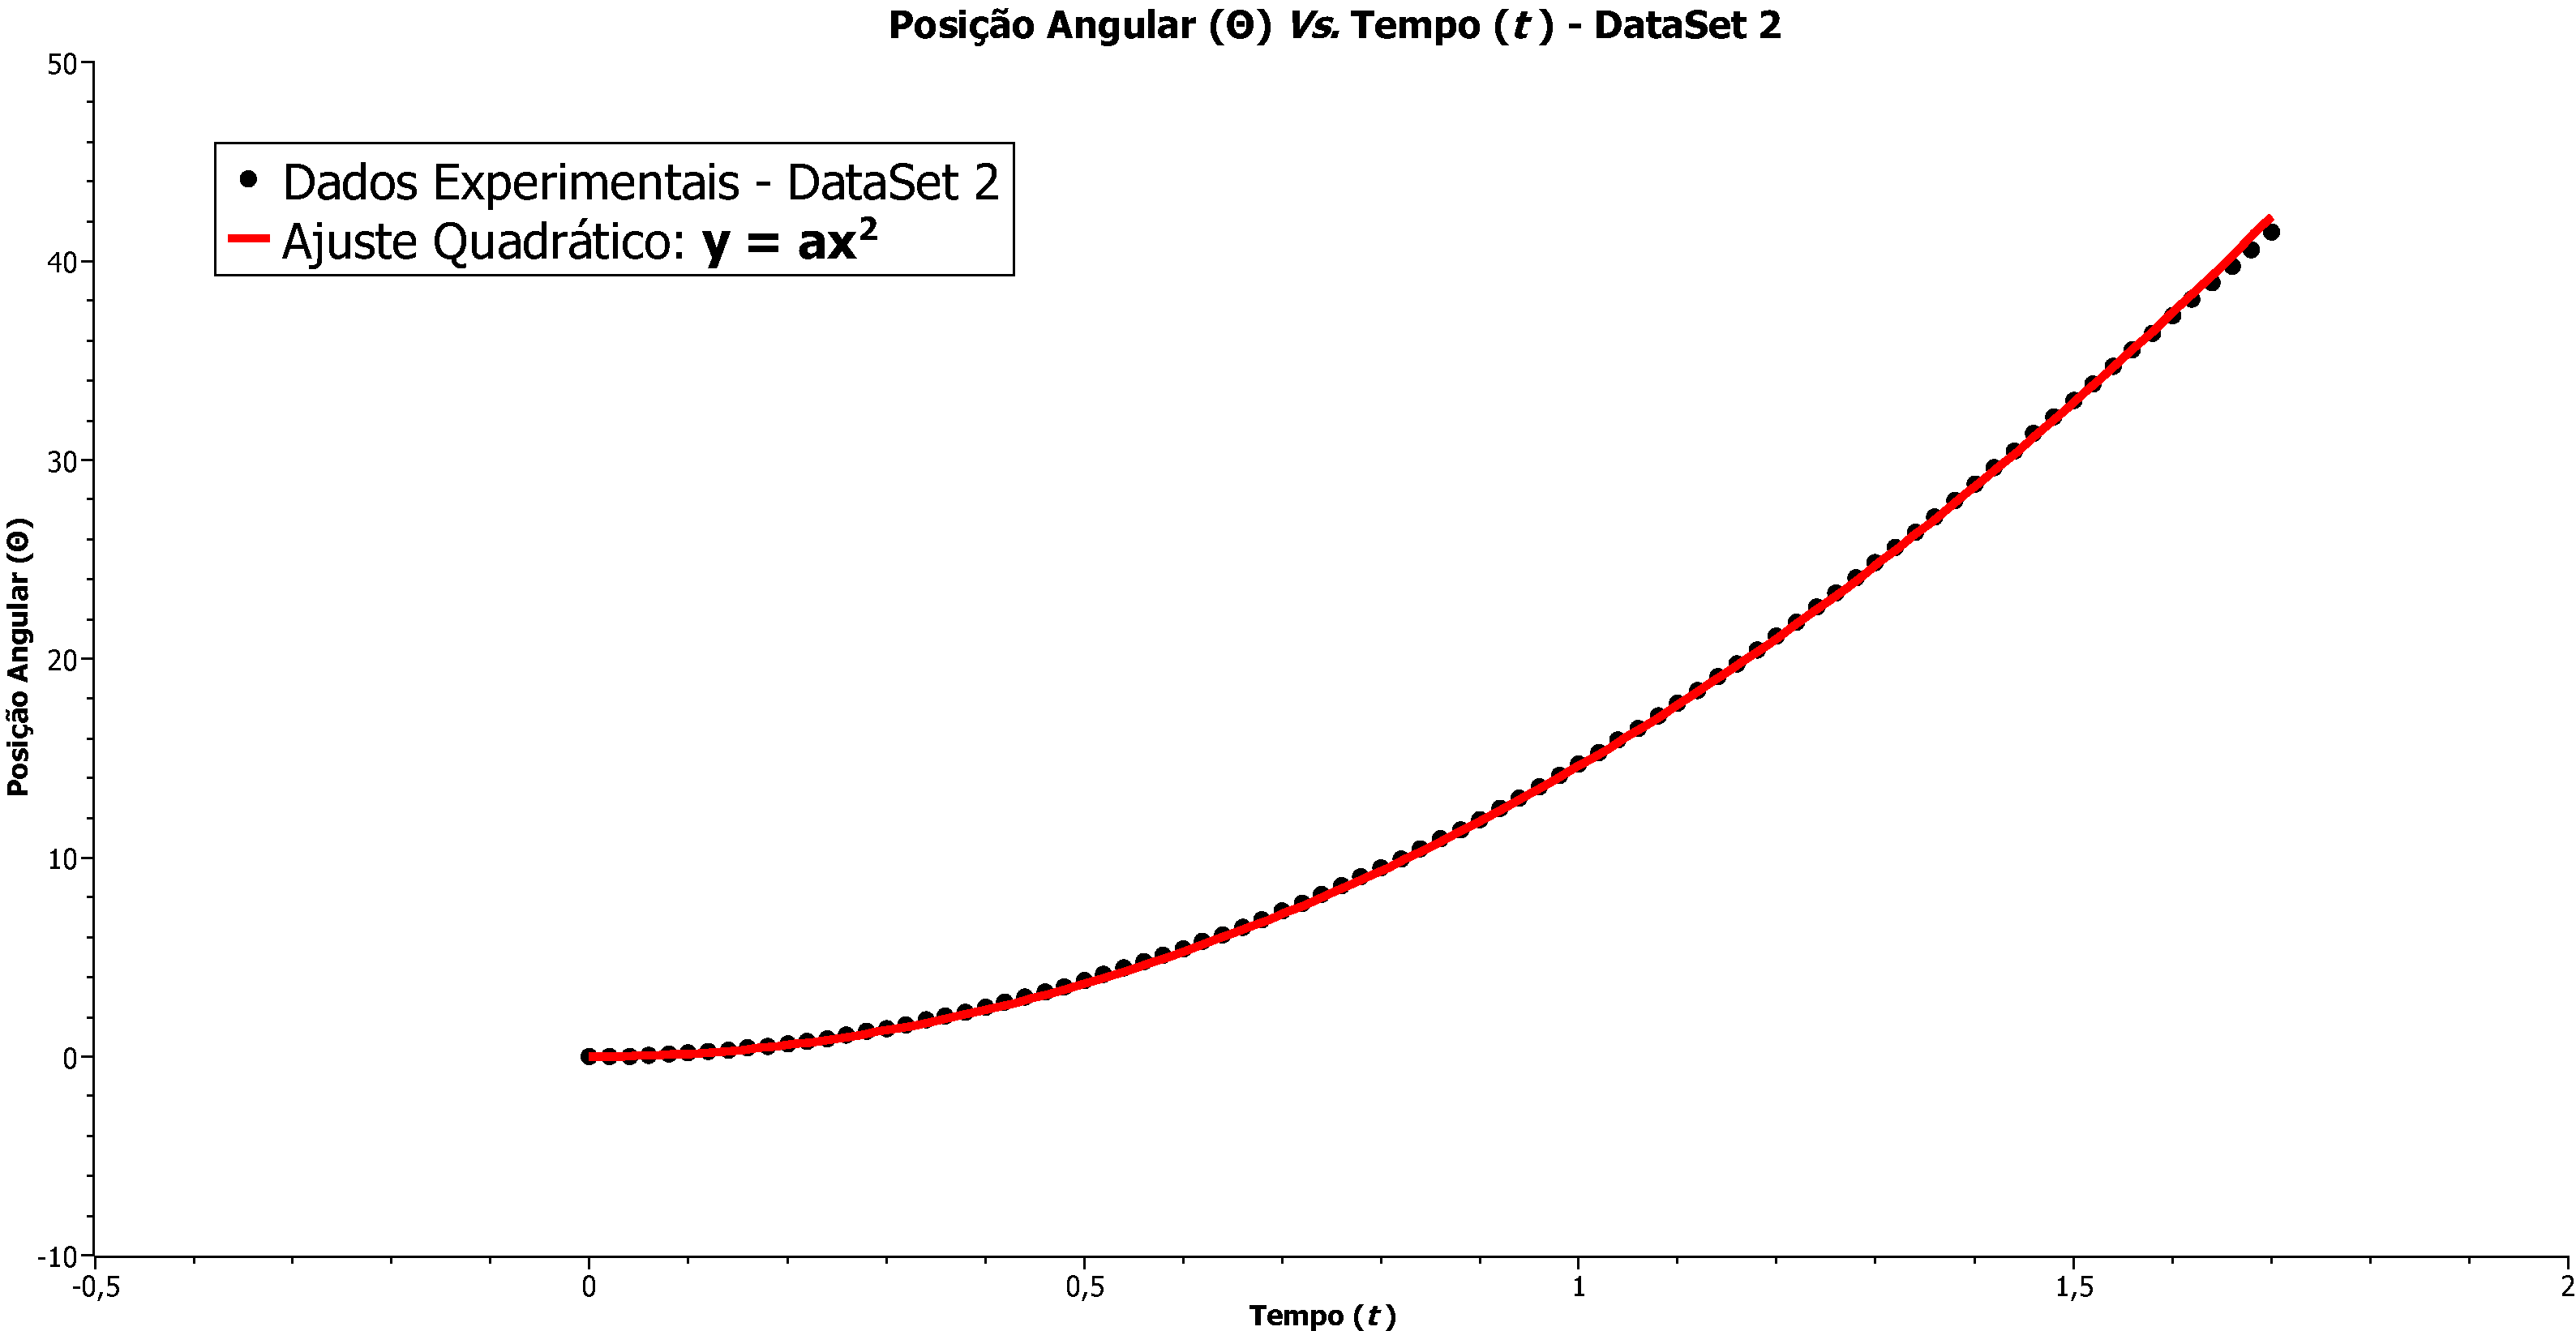
\includegraphics[width=0.9\textwidth]{media/graphs/r2_dataset2}
\caption{Ajuste Linear para o Caso a partir do Repouso - Dataset 1. Fonte: Autor}~\label{fig:ajuste_linear_r2_dataset1}
\end{figure}

O ajuste linear para o caso partindo do repouso resultou no coeficiente $A_{r2} = 14,61 \pm 0,01$.

\subsubsection{Log do SciDAVis}
\begin{verbatim}
[sábado, 18 de abril de 2026 12:05:46 Hora oficial do Brasil	Plot: ''Graph2'']
Non-linear fit of dataset: Table2_Angular Position, using function: a*x^2 + b*x
Y standard errors: Unknown
Scaled Levenberg-Marquardt algorithm with tolerance = 0,0001
From x = 0 to x = 1,43
a  = 14,7966558790166 +/- 0,0451304884196585
b  = 7,52333830919081 +/- 0,0501639128135168
--------------------------------------------------------------------------------------
Chi^2 = 2,19965234028677
R^2 = 0,999960595833728
---------------------------------------------------------------------------------------
Iterations = 1
Status = success
---------------------------------------------------------------------------------------

\end{verbatim}

\subsection{Cálculo do Momento de Inércia Total do Sistema}

Substituindo o valor dos coeficientes $A_{r1}$, $A_{g1}$ e $A_{r1}$ na equação \eqref{eq:moment_inertia_final}, foi possível determinar o momento de inércia do sistema $I_{total}$ para cada um dos 3 coeficientes.

\subsection{Cálculo do Momento de Inércia Total a partir do Ajuste Linear para o caso a partir do Repouso do Dataset 1}

\begin{align}
    I_{total-r1} &= mr_p^2 \left(\frac{g}{2r_p A_{r1}} - 1\right) \nonumber \\
    &= (20,08 \times 10^{-3} \, kg)(23,825 \times 10^{-3} \, m)^2 \left(\frac{9,78 \, m/s^2}{2(23,825 \times 10^{-3} \, m)(21,3)} - 1\right) \nonumber \\
    &= 0,9843 \times 10^{-4} \, kg m^2
\end{align}

\begin{align}
    I_{total-g1} &= mr_p^2 \left(\frac{g}{2r_p A_{g1}} - 1\right) \nonumber \\
    &= (20,08 \times 10^{-3} \, kg)(23,825 \times 10^{-3} \, m)^2 \left(\frac{9,78 \, m/s^2}{2(23,825 \times 10^{-3} \, m)(14,79)} - 1\right) \nonumber \\
    &= 1,467 \times 10^{-4} \, kg m^2
\end{align}

\begin{align}
    I_{total-r2} &= mr_p^2 \left(\frac{g}{2r_p A_{r2}} - 1\right) \nonumber \\
    &= (20,08 \times 10^{-3} \, kg)(23,825 \times 10^{-3} \, m)^2 \left(\frac{9,78 \, m/s^2}{2(23,825 \times 10^{-3} \, m)(14,61)} - 1\right) \nonumber \\
    &= 1,48 \times 10^{-4} \, kg m^2
\end{align}

\subsection{Cálculo do Momento de Inércia da Polia}
Utilizando os momentos total encontrados e o momento de inércia do disco, substituindo os valores na equação \eqref{eq:moment_inertia_polia}, foi possível determinar o momento de inércia da polia $I_{polia}$.

\begin{align}
    I_{polia-r1} &= I_{total-r1} - I_{disco} \nonumber \\
    &= 0,9843 \times 10^{-4} \, kg m^2 - 1,3529 \times 10^{-4} \, kg m^2 \nonumber\\
    &= -3,686 \times 10^{-5} \, kg m^2
\end{align}

\begin{align}
    I_{polia-g1} &= I_{total-g1} - I_{disco} \nonumber \\
    &= 1,467 \times 10^{-4} \, kg m^2 - 1,3529 \times 10^{-4} \, kg m^2 \nonumber\\
    &= 1,141 \times 10^{-5} \, kg m^2
\end{align}

\begin{align}
    I_{polia-r2} &= I_{total-r2} - I_{disco} \nonumber \\
    &= 1,48 \times 10^{-4} \, kg m^2 - 1,3529 \times 10^{-4} \, kg m^2 \nonumber\\
    &= 1,271 \times 10^{-5} \, kg m^2
\end{align}

\subsection{Análise dos Resultados}

Os resultados obtidos para o momento de inércia do sistema ($I_{total}$) e da polia ($I_{polia}$) apresentaram excelente concordância quando comparados o modelo geral do Dataset 1 ($g1$) e o modelo do roteiro aplicado ao Dataset 2 ($r2$). A variação absoluta entre essas duas abordagens válidas foi de apenas $0,13 \times 10^{-5} \, \text{kg}\cdot\text{m}^2$, atestando a repetibilidade do experimento e a estabilidade da inércia da polia na casa de $\approx 1,2 \times 10^{-5} \, \text{kg}\cdot\text{m}^2$.

No entanto, a aplicação estrita do modelo sugerido pelo roteiro ($y = ax^2$) ao Dataset 1 ($r1$) resultou em um momento de inércia negativo para a polia ($-3,686 \times 10^{-5} \, \text{kg}\cdot\text{m}^2$). Sendo essa uma impossibilidade física, a análise minuciosa dos dados brutos desencadeou a hipótese de que o sistema não partiu do repouso absoluto no instante de acionamento do sensor, possuindo uma velocidade angular inicial. Essa condição de contorno forçou o algoritmo de regressão a inflar artificialmente a aceleração para minimizar os erros residuais (fenômeno de \textit{underfitting}). Isso resultou em um coeficiente $A_{r1}$ subestimado, que por sua vez superestimou o termo de aceleração na equação do momento de inércia, levando a um valor negativo para a inércia da polia.

A anomalia foi matematicamente solucionada no caso $g1$, onde a adoção da equação horária completa do movimento ($y = ax^2 + bx$) permitiu isolar a velocidade inicial no termo linear, extraindo a aceleração real do sistema e corrigindo o tensor de inércia para o domínio positivo esperado.

No caso $r2$, a aplicação do modelo do roteiro ao segundo conjunto de dados, que foi coletado com maior cuidado para garantir o repouso inicial, resultou em um valor de inércia da polia positivo e consistente com o modelo geral ($g1$), reforçando a hipótese de que o valor não físico encontrado é resultado de uma falha de laboratório e que a condição de contorno inicial é crucial para a validade do modelo simplificado proposto.

\section{Discussão}

A análise dos resultados revelou que a escolha do modelo de ajuste linear tem um impacto significativo na determinação do momento de inércia da polia. O modelo simplificado, que assume um movimento a partir do repouso absoluto, pode levar a resultados não físicos se essa condição não for rigorosamente atendida. Por outro lado, o modelo geral, que inclui um termo para a velocidade inicial, mostrou-se mais robusto e capaz de fornecer resultados consistentes mesmo quando a condição de repouso absoluto não foi estritamente observada.

A comparação entre os resultados dos dois conjuntos de dados reforça a importância de garantir condições de contorno adequadas durante a coleta de dados experimentais, especialmente em sistemas dinâmicos onde a velocidade inicial pode influenciar significativamente os resultados. 

Além disso, a análise destaca a necessidade de uma abordagem crítica na interpretação dos resultados experimentais, considerando as limitações dos modelos teóricos e as possíveis fontes de erro na coleta de dados.

\section{Conclusão}

O experimento permitiu a determinação do momento de inércia da polia, utilizando dois conjuntos de dados e dois modelos de ajuste linear. Os resultados indicaram que o modelo geral, que inclui um termo para a velocidade inicial, é mais adequado para a análise do sistema, especialmente quando a condição de repouso absoluto não é garantida. Mas o modelo simplificado, é bastante eficaz uma vez que as condições de contorno são atendidas. A análise dos resultados destacou a importância de considerar as condições de contorno e as limitações dos modelos teóricos na interpretação dos dados experimentais.

\bibliographystyle{plainnat}
\bibliography{refs}

\end{document}